\chapter{Transporte óptimo entre distribuciones}
\label{ot}

En este capítulo se revisarán algunos conceptos y resultados fundamentales del transporte óptimo, un campo esencial dentro de la ingeniería y la matemática aplicada que últimamente ha ganado un gran interés en la comunidad del aprendizaje de máquinas y, en particular, de los modelos generativos. Desde un punto de vista práctico, el tipo de problemas de optimización que busca resolver el transporte óptimo pueden ser adaptados a una infinidad de contextos diferentes, permitiendo utilizar resultados importantes de la teoría en la toma de decisiones en escenarios complejos. Por otra parte, desde un punto de vista teórico, el transporte óptimo es un área bien estudiada desde la matemática, permitiendo obtener garantías teóricas y propiedades e interpretaciones geométricas relevantes.

Antes de conectar el transporte óptimo con los modelos de difusión y ver las ventajas que esto implica, se comenzará estudiando el transporte óptimo de forma general, sin limitar su aplicación a los modelos generativos. Posteriormente, en la \autoref{ot/dynamic/dm} se conectará el transporte óptimo con los modelos de difusión y se verá que los modelos de difusión, en el mejor de los casos, resuelven un caso particular de transporte óptimo.

Con el fin de construir los problemas de transporte óptimo de una forma más natural, primero serán motivados en su versión discreta y luego generalizados a su versión continua en $\R^d$. Esto permite obtener resultados de manera sencilla al trabajar en el caso discreto, los cuales después serán extendidos al caso continuo sin demostración. Además, es importante mencionar que tener un entendimiento más acabado de las formulaciones discretas es más beneficioso al momento de realizar implementaciones numéricas, las que constituyen gran parte de las aplicaciones del transporte óptimo.

Por otra parte, de aquí en adelante ya no se asumirá que las medidas de probabilidad poseen una función de densidad (ver \autoref{measure_theory/density}) al trabajar en formulaciones continuas dado que esta suposición solo limita el alcance de los problemas de transporte óptimo y no aporta significativamente a la simplificación de la teoría. Además, cuando se hable de \textit{solución} de un problema de optimización, se estará haciendo referencia a un elemento del conjunto factible que alcance el valor ínfimo de la función objetivo (i.e., que sea un mínimo)\footnote{Recordar que la existencia del valor ínfimo para un problema de optimización no garantiza a priori la existencia de una solución. Considerar, por ejemplo, un problema de optimización donde el conjunto factible es un conjunto abierto y el valor ínfimo del problema de optimización se alcanza en la frontera del conjunto factible.}. En consecuencia, todos los problemas serán escritos utilizando $\inf$ (resp. $\sup$) en vez de $\min$ (resp. $\max$), esto con el fin de mostrar el mérito de los resultados de existencia de soluciones.

Para introducir el problema de transporte óptimo, se propone considerar dos conjuntos finitos $\xspace=\{x_i\}_{i=1}^n$ e $\yspace=\{y_j\}_{j=1}^m$, por ahora con $n=m$, donde el objetivo es encontrar una biyección $T:\xspace\to\yspace$ que minimice algún funcional de costo, el cual suele ser una suma de costos individuales de emparejamiento\footnote{Notar que este problema es equivalente al problema de buscar un matching óptimo en un grafo bipartito cuyas particiones son $\xspace$ e $\yspace$. Equivalentemente, las soluciones pueden identificarse con permutaciones del conjunto $\{1,\ldots,n\}.$}. Con esta idea, dado $c:\xspace\times\yspace\to\R$, donde $c(x_i,y_j)$ indica el costo de emparejar $x_i$ con $y_j$, el problema de optimización se plantea de la siguiente forma:

\begin{equation}
	\label{eq:ot_motivation}
	\inf_{\feasible{T:\xspace\to\yspace}{T\text{es biyección}}}
	\sum_{i=1}^n c\left(x_i,T(x_i)\right).
\end{equation}

Notar que el conjunto de biyecciones es finito y no vacío cuando $n=m$, por lo que este problema siempre tiene solución (aunque no necesariamente es única). Por otra parte, es importante indicar que el funcional de costo discreto $c:\xspace\times\yspace\to\R$ siempre se puede identificar con una matriz $C\in\matrixspace{n,m}{\R}$ mediante $C_{ij}=c(x_i,y_j)$.

Para ilustrar este problema en el área del aprendizaje automático, se puede considerar el problema de asignar particiones de datos de entrenamiento a diferentes GPUs para realizar un entrenamiento distribuido. En este escenario, $\xspace$ representa el conjunto de particiones de datos, mientras que $\yspace$ representa el conjunto de GPUs disponibles para el entrenamiento. Para la función de costo se podría considerar buscar una asignación que minimice la suma del tiempo total de transporte de datos para cada par partición-GPU, $(x,T(x))\in\xspace\times\yspace$, que asigne el mapa $T$.

Si bien esta formulación es lo suficientemente general como para ser utilizada en diferentes problemas, también tiene múltiples desventajas. La primera de ellas es que al ser un problema de optimización discreto, debe ser tratado como un problema combinatorial, siendo difícil de resolver para valores muy grandes de $n=m$ ya que el conjunto factible tiene $n!$ elementos. Además, esta formulación no tiene solución en casos donde $\xspace$ e $\yspace$ tienen distinto cardinal (ya que no es posible construir una biyección) y no permite asociar varios elementos de $\xspace$ a un mismo elemento de $\yspace$, lo cual es útil, por ejemplo, si las GPUs tienen suficiente memoria en el problema de entrenamiento distribuido.

Para resolver estas limitaciones, en la \autoref{ot/monge} se relajará la formulación anterior permitiendo asignar varios elementos de $\xspace$ a un mismo elemento de $\yspace$, obteniendo versión más general del problema \eqref{eq:ot_motivation} conocida como \textit{problema de Monge}. Posteriormente, en la \autoref{ot/kantorovich} se mostrarán algunas dificultades de este nuevo enfoque, por lo que se modificará el problema de Monge para obtener la \textit{relajación de Kantorovich}, la cual es otro problema de optimización que tiene buenas propiedades tanto teóricas como prácticas y que, bajo ciertas condiciones, es equivalente al problema de Monge. Posteriormente, en la \autoref{ot/dynamic} se incluirá la variable temporal en estos problemas para dar una interpretación dinámica del problema de transporte óptimo, la cual, en particular, será comparada con los modelos de difusión en la \autoref{ot/dynamic/dm} y luego generalizada a una versión estocástica en el \autoref{eot_sbp}, la cual resultará ser equivalente al problema del puente de Schrödinger.

Para poder realizar el estudio del transporte óptimo, son necesarias algunas definiciones elementales de teoría de la medida, las cuales se pueden encontrar, por completitud, en el \autoref{measure_theory}.

\section{Problema de Monge}
\label{ot/monge}

Si bien el problema de la infactibilidad del problema \eqref{eq:ot_motivation} para $n\neq m$ se puede solucionar eliminando la restricción de biyectividad para $T$\footnote{En particular, pidiendo solo sobreyectividad se soluciona la infactibilidad para $n>m$ mientras que pidiendo solo inyectividad se soluciona la infactibilidad para $n<m$.}, el problema sigue teniendo la limitación de tratar a todos los elementos de $\xspace$ e $\yspace$ por igual. En el problema de entrenamiento distribuido, esto implica que el problema \eqref{eq:ot_motivation} no es consciente de atributos relevantes como el tamaño de la partición o la capacidad de la GPU. Para resolver limitaciones de este tipo, se modificará el marco de trabajo del problema anterior y se considerará adicionalmente que cada elemento $x_i\in\xspace$ tiene asignado un valor $a_i\in\R$ que podrá ser usado dentro de la función de costo. Similarmente, cada elemento $y_j\in\yspace$ tendrá asignado un valor $b_j\in\R$.

\subsection{Formulación del problema}
\label{ot/monge/formulation}

El problema de Monge será introducido en su versión discreta y luego generalizado a su versión continua en $\R^d$. De aquí en adelante, ya no se considerará la restricción $n=m$.

\subsubsection{Formulación discreta}

Con el fin de mostrar otra perspectiva del transporte óptimo, se motivará el problema de Monge usando el clásico problema de asignación de recursos mineros. En este escenario, una compañía posee un conjunto $\xspace=\{x_i\}_{i=1}^n$ de yacimientos mineros, donde cada yacimiento $x_i\in\xspace$ produce una cantidad $a_i>0$ de cierta materia prima. Por otra parte, un conjunto de fábricas $\yspace=\{y_j\}_{j=1}^m$ espera recibir una cantidad $b_j>0$ en cada una de las fábricas $y_j\in\yspace$, pudiendo abastecerse de diferentes yacimientos de $\xspace$\footnote{La restricción $a_i,b_j>0$ no limita la generalidad del problema ya que si algún $a_i$ (resp. $b_j$) fuese nulo, se podría eliminar de la familia $\xspace$ (resp. $\yspace$) el punto $x_i$ (resp. $y_j$) asociado.}. El problema de transporte óptimo aquí consiste en satisfacer la demanda de todas las fábricas minimizando el costo de transportar la materia prima desde los yacimientos mineros hacia las fábricas.

Bajo este marco, el problema de asignar la oferta de $\xspace$ entre la demanda de $\yspace$ minimizando un funcional de transporte $c:\xspace\times\yspace\to\R$ se formula de la siguiente forma:

\begin{equation}
	\label{eq:monge_no_measure}
	\inf_{T:\xspace\to\yspace} \sum_{i=1}^n c\left(x_i,T(x_i)\right)
	\quad\text{s.a}\quad
	\sum_{i\,:\,T(x_i)=y_j} a_i = b_j ,\quad\forall j\in\{1,\ldots,m\},
\end{equation}

donde la restricción adicional busca que se cumpla la demanda para cada $y_j\in \yspace$. Es importante notar que en esta restricción, la suma es sobre (la oferta de) los elementos de $\xspace$ que envían masa a $y_j$, es decir, el conjunto $T^{-1}(\{y_j\})=\{x_i\in\xspace:T(x_i)=y_j\}$.

Notar que el mapa buscado $T$ ya no necesita ser biyectivo pero sí es necesariamente sobreyectivo ya que, de lo contrario, de acuerdo a la restricción, habría un $b_j=0$, lo cual contradice que $\{b_j\}_{j=1}^m\subset\R_{++}$. Por otra parte, al considerar $n=m$ y $a=b=\1$, se recupera la biyectividad de $T$ y la restricción se cumple trivialmente, concluyendo que \eqref{eq:ot_motivation} es un caso particular del problema \eqref{eq:monge_no_measure}.

Por otra parte, la solución no tiene por qué existir ni ser única: la sobreyectividad de $T$ no se puede alcanzar cuando $n<m$, por lo que en este caso el problema es infactible y no hay solución. Sin embargo, se verá que para el caso $n=m$ sí existe solución cuando la cantidad ofertada total es igual a la cantidad demandada total. Por otro lado, en algunos casos es posible encontrar varias soluciones cuando el problema presenta algún tipo de simetría.

Si bien la formulación del problema \eqref{eq:monge_no_measure} es bastante clara, es usual escribir el problema como un problema de transporte entre medidas de probabilidad\footnote{Si bien en el caso discreto no son evidentes las ventajas de esta formulación, sí se vuelve más natural al estudiar el problema de Kantorovich en la \autoref{ot/kantorovich}.}. Bajo este enfoque, los elementos de $\xspace$ se interpretarán como puntos en un espacio medible discreto (ver \autoref{measure_theory/definition/discrete}), mientras que los vectores $a=(a_1,\ldots,a_n)^\top$ y $b=(b_1,\ldots,b_m)^\top$ representarán medidas discretas en dichos espacios.

Para poder considerar únicamente medidas de probabilidad, se pedirá que los vectores $a\in\R^n$ y $b\in\R^m$ sean vectores de probabilidad\footnote{Esto no limita el alcance de la formulación ya que cualquier vector $v\in\R_+^d$ puede ser normalizado al simplex $\Sigma_d$.} (i.e., $a\in\Sigma_n$ y $n\in\Sigma_m$, donde $\Sigma_n$ está definido en \eqref{eq:simplex}). Con estas observaciones, se construyen las medidas discretas $\mu\in\probmeasure{\xspace}$ y $\nu\in\probmeasure{\yspace}$ definidas como:

\begin{equation*}
	\mu = \sum_{i=1}^n a_i \delta_{x_i} \qquad
	\nu = \sum_{j=1}^m b_i \delta_{y_j}.
\end{equation*}

Bajo esta interpretación, \eqref{eq:monge_no_measure} se entiende como el problema de buscar un mapa $T:\xspace\to\yspace$ que transporte de forma óptima la distribución masa $\mu$ de los elementos de $\xspace$ hacia una distribución de masa $\nu$ en $\yspace$. Por otra parte, la restricción en \eqref{eq:monge_no_measure} se interpreta como una condición de preservación de medida después del transporte, donde la masa de cada elemento $y_j\in\yspace$ debe ser igual a la masa total de todos los elementos $x_i\in\xspace$ que fueron transportados hacia $y_j$. En el enfoque de teoría de la medida, esta restricción indica precisamente que $T_\#\mu=\nu$ (ver \autoref{defn:push_forward}), donde la medida push-forward $T_\#\mu\in\probmeasure{\yspace}$ toma la siguiente forma en el caso discreto:

\begin{equation}
	\label{eq:push_forward_discrete}
	T_\#\mu := \sum_{i=1}^n a_i \delta_{T(x_i)}.
\end{equation}

Observar que esta medida transforma el vector de probabilidad $a\in\Sigma_n$ asociado a $\mu$ en un vector de probabilidad en $\Sigma_m$ cuya $j$-ésima coordenada es $\sum_{i:T(x_i)=y_j} a_i$. Con esta nueva notación se puede formular lo que se conoce como el problema de Monge:

\begin{defn}[problema de Monge, versión discreta]
	Dados dos conjuntos finitos, $\xspace=\{x_i\}_{i=1}^n$ e $\yspace=\{y_j\}_{j=1}^m$, y dos medidas de probabilidad $\mu\in\probmeasure{\xspace}$ y $\nu\in\probmeasure{\yspace}$ con vectores de probabilidad $a\in\Sigma_n$ y $b\in\Sigma_m$ respectivamente, el problema de Monge entre $\mu$ y $\nu$ para un funcional de costo $c:\xspace\times\yspace\to\R$ es:

	\begin{equation}
		\label{eq:monge_discrete}
		\inf_{\feasible{T:\xspace\to\yspace}{T_\#\mu=\nu}}
		\sum_{i=1}^n c(x_i,T(x_i)).
	\end{equation}

	Además, a una solución óptima $T^*$ del problema \eqref{eq:monge_discrete}, en caso de existir, se le denomina \textit{mapa de Monge}.
\end{defn}

Como este problema es solo una reformulación del problema \eqref{eq:monge_no_measure}, la existencia de un mapa $T:\xspace\to\yspace$ que satisfaga $T_\#\mu = \nu$ no es segura y la solución del problema, en caso de existir, no tiene por qué ser única. Sin embargo, cuando $n=m$ y las medidas $\mu$ y $\nu$ son uniformes (i.e., $a=b=\frac{1}{n}\1$), se puede demostrar que el problema \eqref{eq:monge_discrete}, equivalente en este caso al problema de matching \eqref{eq:ot_motivation}, posee solución (ver \autoref{prop:matching_existence}).

\subsubsection{Formulación continua}

El problema de Monge discreto \eqref{eq:monge_no_measure} (o \eqref{eq:monge_discrete} en su versión medible) puede ser extendido a un problema de transporte continuo, donde se busca trasladar una cierta cantidad de masa, no necesariamente puntual, de un lugar a otro. Para motivar su formulación es usual considerar el problema de trasladar eficientemente un montículo de tierra con una forma y densidad específica hacia otro lugar con una forma y densidad no necesariamente igual a la original. Este problema se ilustra en la \autoref{fig:ot/earth_mover}.

\insertimage{ot/earth_mover}{0.8}{Problema del transporte de tierra, donde el montículo rojo (con densidad de masa $\rho_1$) debe ser trasladado al montículo azul (con densidad de masa $\rho_2$). Para un mapa de transporte $T$, un volumen $A\subset\xspace$ es transportado hacia el volumen $T(A)=\{T(x):x\in A\}\subset\yspace$. Inversamente, un volumen $B\subset\yspace$ es formado por la tierra proveniente de $T^{-1}(B)=\{x\in A:T(x)\in B\}\subset\xspace$. Notar que la masa de un volumen $A\subset\xspace$ se puede calcular mediante $m_1(A)=\int_A \rho_1(x)\d x$ (análogo para $\yspace$). Esta figura se puede encontrar en el archivo \texttt{earth\_mover.ipynb}.}

En este caso, el problema de transporte consiste en encontrar un mapa de transporte $T:\xspace\to\yspace$ (con $\xspace=\yspace=\R^2)$ que minimice un cierto costo de transporte (p.g. la distancia recorrida durante el transporte) pero que también respete una condición de preservación de masa. Para esto último, es necesario, al igual que en el caso discreto, exigir que la masa de cada volumen de tierra $B\subset\R^2$ en el montículo de destino sea igual a la masa total que llega desde el montículo de origen hacia $B$. En consecuencia, si los montículos de origen y destino tienen densidades de masa $\rho_1,\rho_2:\R^2\to\R_+$ respectivamente, el mapa de transporte $T$ debe cumplir

\begin{equation}
	\label{eq:push_forward_r2}
	\int_{B} \rho_2(y) \d y = \int_{T^{-1}(B)} \rho_1(x) \d x,
	\quad\forall B\in\borel{\yspace},
\end{equation}

donde $T^{-1}(B) = \{x\in\xspace : T(x)\in B\}\in\borel{\xspace}$ es el volumen de masa en el montículo de origen que es transportado hacia $B$ y $\borel{\xspace}$ (resp. $\borel{\yspace}$) es el conjunto de conjuntos medibles en $\xspace$ (resp. $\yspace$; ver \autoref{defn:sigma_algebra}). Notar que esta restricción es análoga a la restricción del problema discreto \eqref{eq:monge_no_measure}. Además, considerando las funciones de masa $m_1(A) := \int_A \rho_1(x)\d x$ y $m_2(B) := \int_B \rho_2(y)\d y$, se vuelve claro que la condición \eqref{eq:push_forward_r2} es una condición de preservación de masa:

\begin{equation}
	\label{eq:monge_earth_mass}
	m_2(B) = m_1\parent{T^{-1}(B)},
	\quad\forall B\in\borel{\yspace}.
\end{equation}

Al igual que en la formulación discreta, es posible interpretar las funciones de masa $m_1$ y $m_2$ como medidas (en este caso en $\R^2$) $\mu$ y $\nu$ respectivamente donde, además, se observa que la existencia de las densidades $\rho_1$ y $\rho_2$ no es necesaria para la formulación ya que se puede trabajar directamente con la restricción \eqref{eq:monge_earth_mass} en vez de \eqref{eq:push_forward_r2}. En ambos casos, la condición de conservación de masa en \eqref{eq:monge_earth_mass} o \eqref{eq:push_forward_r2} se denota, al igual que en el caso discreto, como $T_\#m_1 = m_2$, donde $T_\# m_1\in\probmeasure{\yspace}$ es la medida push-forward inducida por $m_1$ a través de $T$.

Esto motiva a construir la siguiente definición, la cual también es válida en el caso discreto:

\begin{defn}[mapa de transporte]
	Una función $T:\xspace\to\yspace$ es un \textit{mapa de transporte} entre dos medidas de probabilidad $\mu\in\probmeasure{\xspace}$ y $\nu\in\probmeasure{\yspace}$ si $T_\#\mu = \nu$.
	
	Equivalentemente, si se tienen dos variables aleatorias con $x\sim\mu$ e $y\sim\nu$, entonces $T$ es un mapa de transporte si $y=T(x)$.
\end{defn}

Notar que en el caso discreto es posible escribir explícitamente la medida push-forward $T_\#\mu$ de acuerdo a \eqref{eq:push_forward_discrete}. En la \autoref{prop:push_forward_properties} se encuentran algunas propiedades del operador push-forward en el caso general. Con esta reinterpretación, el problema de Monge toma la siguiente forma en su versión continua:

\begin{defn}[problema de Monge, versión continua]
	Dados los conjuntos $\xspace\subset\R^n$ e $\yspace\subset\R^m$, el problema de Monge entre dos medidas de probabilidad, $\mu\in\probmeasure{\xspace}$ y $\nu\in\probmeasure{\yspace}$, asociado a un funcional de costo integrable $c:\xspace\times\yspace\to\R$ es:

	\begin{equation}
		\label{eq:monge_continuous}
		\inf_{\feasible{T:\xspace\to\yspace}{T_\#\mu=\nu}}
		\int_{\xspace} c(x, T(x)) \d\mu(x).
	\end{equation}

	Además, a una solución óptima $T^*$ del problema \eqref{eq:monge_continuous}, en caso de existir, se le denomina \textit{mapa de Monge}.
\end{defn}

Notar que el conjunto factible es precisamente el conjunto de mapas de transporte. Por otra parte, cuando las medidas $\mu\in\probmeasure{\xspace}$ y $\nu\in\probmeasure{\yspace}$ tienen funciones de densidad $p_\mu$ y $p_\nu$ respectivamente (ver \autoref{teo:radon_nikodym}), el problema \eqref{eq:monge_continuous} se puede reescribir como:

\begin{equation*}
	\inf_{\feasible{T:\xspace\to\yspace}{T_\#\mu=\nu}}
	\int_{\xspace} c(x, T(x))\, p_\mu(x)\d x ,
\end{equation*}

donde, de acuerdo a la \autoref{prop:push_forward_characterization}, la restricción $T_\#\mu=\nu$ equivale a:

\begin{equation*}
	\int_\yspace h(y)\, p_\nu(y) \d y = \int_\xspace h(T(x))\, p_\mu(x) \d x,
	\quad\forall h\in \continuous{\yspace} ,
\end{equation*}

donde $\continuous{\yspace}$ es el conjunto de funciones $f:\yspace\to\R$ continuas.

En la próxima sección se verán limitaciones de este problema y se estudiará una formulación alternativa para el problema de transporte óptimo, la cual tendrá mejores propiedades tanto teóricas como prácticas.

\section{Relajación de Kantorovich}
\label{ot/kantorovich}

Si bien el problema de Monge es más general que el problema inicial \eqref{eq:ot_motivation}, no tiene propiedades deseables como ser un problema de optimización convexo. En efecto, en el caso continuo con $\xspace=\yspace=\R^d$, si las medidas $\mu$ y $\nu$ poseen funciones de densidad $p_\mu$ y $p_\nu$ respectivamente, se puede demostrar que la restricción $T_\#\mu=\nu$ es equivalente a que se cumpla la ecuación $p_\mu(x) = p_\nu(T(x))\left|\det\parent{\nabla_x T(x)}\right|$, la cual es altamente no lineal.

En esta sección se relajará el problema de Monge, permitiendo repartir la masa de los elementos de $\xspace$ en múltiples elementos de $\yspace$, lo cual se puede interpretar como una asignación probabilística para el problema de transporte de Monge. Este nuevo problema, en su versión discreta, tendrá la propiedad de ser convexo y, más importante aún, permitirá definir una métrica en (un subconjunto de) el espacio de medidas de probabilidad, $\probmeasure{\xspace}$.

\subsection{Formulación primal}
\label{ot/kantorovich/primal}

Al igual que para el problema de Monge, el problema de Kantorovich será formulado inicialmente en una versión discreta y luego extendido a su formulación continua. Además, al ser un problema de optimización convexo, será natural estudiar su problema dual, lo cual se realizará en la \autoref{ot/kantorovich/dual}.

\subsubsection{Problema discreto}

En el problema de transporte de materia prima introducido anteriormente, es razonable considerar que un mismo yacimiento pueda enviar parte de su materia prima a distintas fábricas, lo cual no está permitido en la formulación discreta del problema de Monge, \eqref{eq:monge_discrete}. Notar que esta relajación es análoga a la realizada en el problema de Monge donde, a diferencia del problema inicial \eqref{eq:ot_motivation}, se permitió que elementos de $\yspace$ estén enlazados a más de un elemento de $\xspace$.

Sin embargo, permitir una asignación múltiple cambia considerablemente el problema de Monge discreto \eqref{eq:monge_discrete}. En efecto, el mapa buscado $T:\xspace\to\yspace$ deja de ser una función, perdiendo todas las propiedades que esto implicaba. Es por este motivo que para formular este nuevo problema, ahora se buscará una función $\tilde T:\xspace\times\yspace\to\R_+$, donde $\tilde T(x,y)$ indica la cantidad de masa que se transportará desde $x\in\xspace$ hacia $y\in\yspace$. Dado que se está en un marco discreto, esto es equivalente a buscar una matriz de transporte $P\in\matrixspace{n,m}{[0,1]}$ donde $P_{ij}$ indica la cantidad de masa que se debe trasladar desde $x_i\in\xspace$ hacia $y_j\in\yspace$.

Por otra parte, es necesario que la matriz de transporte $P$ respete la conservación de masa (equilibrio oferta-demada) tanto en la medida de origen $\mu\in\probmeasure{\xspace}$ como en la medida de destino $\nu\in\probmeasure{\yspace}$. En el problema de transporte desde yacimientos hacia fábricas, la $i$-ésima fila de la matriz $P$ representa cómo se reparte la materia prima de $x_i\in\xspace$, por lo que se debe imponer que la suma de dicha fila sea igual al valor $a_i\in[0,1]$. Del mismo modo, la $j$-ésima columna de $P$ representa la cantidad de materia prima que llega a la fábrica $y_j\in\yspace$, por lo que la suma de dicha columna debe ser igual a $b_j\in[0,1]$.

Por último, para formular el problema de forma clara, el funcional de costo $c:\xspace\times\yspace\to\R$ usado en el problema de Monge \eqref{eq:monge_discrete} se identificará con una matriz $C\in\matrixspace{n,m}{\R}$ mediante $C_{ij}=c(x_i,x_j)$, por lo que $C_{ij}\in\R$ indica el costo de transportar una unidad de masa desde $x_i\in\xspace$ hacia $y_j\in\yspace$. De esta forma, el costo total de transporte consistirá en el producto Frobenius entre la matriz de asignación de masa $P\in\matrixspace{n,m}{[0,1]}$ y la matriz de costo $C\in\matrixspace{n,m}{\R}$:

\begin{defn}[problema de Kantorovich, caso discreto]
	Dados dos conjuntos finitos, $\xspace=\{x_i\}_{i=1}^n$ e $\yspace=\{y_j\}_{j=1}^m$, y dos medidas de probabilidad $\mu\in\probmeasure{\xspace}$ y $\nu\in\probmeasure{\yspace}$ con vectores de probabilidad $a\in\Sigma_n$ y $b\in\Sigma_m$ respectivamente, el problema de Kantorovich entre $\mu$ y $\nu$ para una matriz de costo $C\in\matrixspace{n,m}{\R}$ es:

	\begin{equation}
		\label{eq:kantorovich_discrete}
		\inf_{P\in \Pi_d(\mu,\nu)} \dotproduct{C}{P}_F := \sum_{i=1}^{n}\sum_{j=1}^{m} C_{ij}P_{ij} ,
	\end{equation}

	donde la región factible $\Pi_d(\mu,\nu)$ se define como:

	\begin{equation*}
		\Pi_d(\mu,\nu) := \left\{P\in\matrixspace{n,m}{[0,1]}\,:\,
		\sum_{j=1}^m P_{ij} = a_i,\, \forall i\in\{1,\ldots,n\},\quad
		\sum_{i=1}^n P_{ij} = b_j,\, \forall j\in\{1,\ldots,m\}
		\right\}.
	\end{equation*}

	Además, a una solución óptima $P^*$ del problema \eqref{eq:kantorovich_discrete}, en caso de existir, se le denomina \textit{plan de Kantorovich}.
\end{defn}

A modo de ejemplo, en la \autoref{fig:ot/kantorovich_discrete_example} se puede ver la solución para un problema de transporte discreto específico.

\begin{figure}
	\centering
	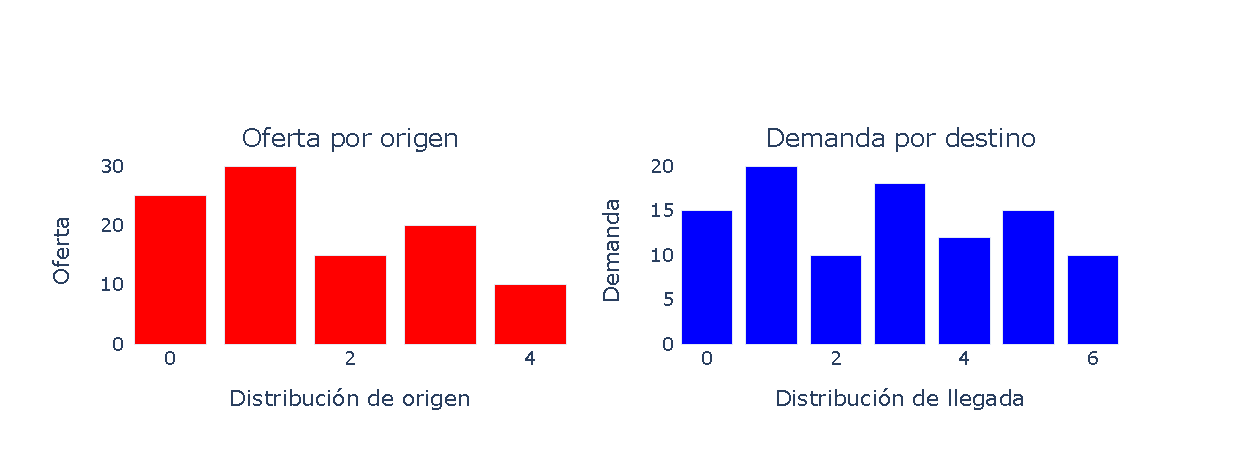
\includegraphics[width=0.8\textwidth]{images/ot/kantorovich_discrete_histogram}

	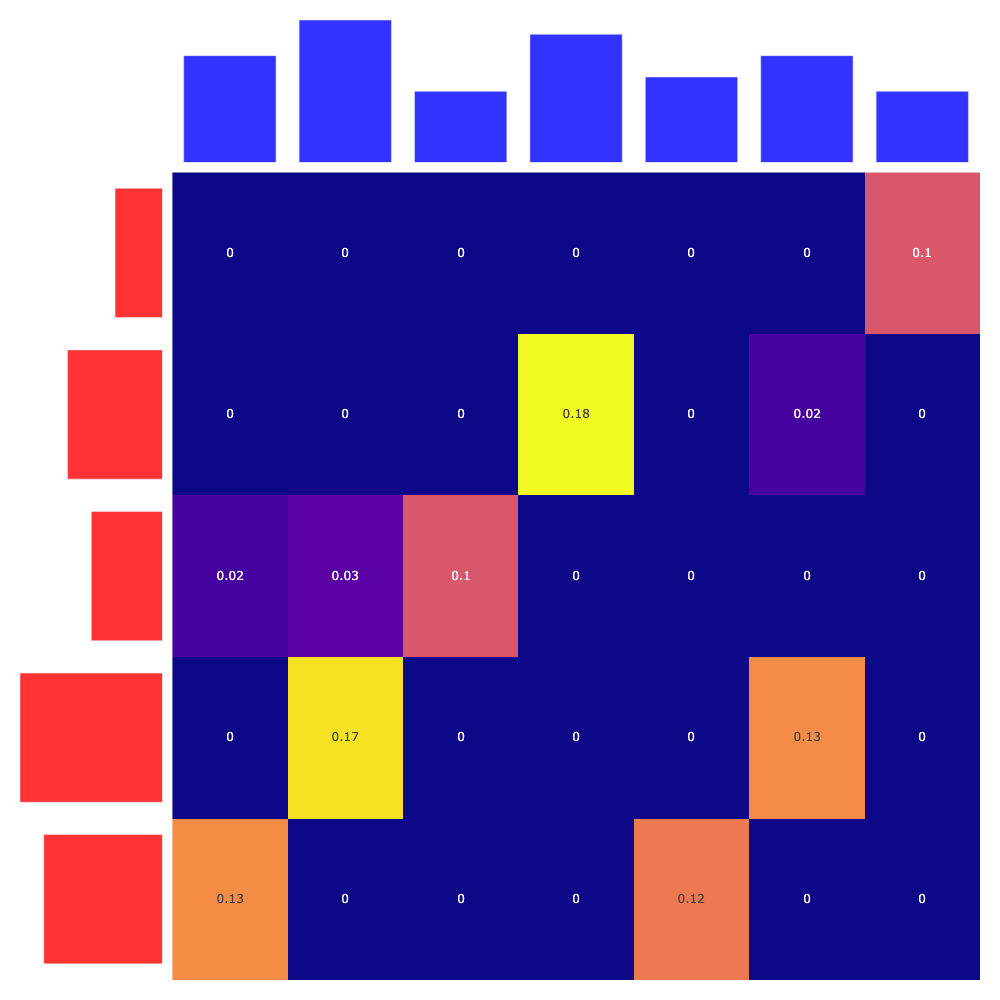
\includegraphics[width=0.5\textwidth]{images/ot/kantorovich_discrete_solution}
	\caption{(Arriba) histogramas discretos (no normalizados) asociados a las medidas $\mu$ y $\nu$ respectivamente, donde $|\xspace|=5$ y $|\yspace|=7$. (Abajo) solución (normalizada) para el problema de Kantorovich entre las dos distribuciones discretas. El código de esta simulación se encuentra en el archivo \texttt{kantorovich.ipynb}.}
	\label{fig:ot/kantorovich_discrete_example}
\end{figure}

Notar que el conjunto $\Pi_d(\mu,\nu)$ es no vacío (por lo que el problema de optimización siempre es factible) ya que siempre se puede considerar la matriz $P\in\matrixspace{n,m}{[0,1]}$ definida como $P_{ij}=a_ib_j$, la cual pertenece a $\Pi_d(\mu,\nu)$. En efecto, dado que $a\in\Sigma_n$ y $b\in\Sigma_m$:

\begin{equation*}
	\sum_{j=1}^m P_{ij} = a_i\sum_{j=1}^m b_j = a_i,\, \forall i\in\{1,\ldots,n\},
	\quad
	\sum_{i=1}^n P_{ij} = b_j\sum_{i=1}^n a_i = b_j,\, \forall j\in\{1,\ldots,m\}.
\end{equation*}

Más adelante será útil recordar que esta matriz se puede escribir como $P=ab^\top$. Por otra parte, la restricción de conservación de masa para $\mu$ se puede escribir vectorialmente como $P\1_{m}=a$, mientras que para $\nu$, se puede escribir como $P^\top \1_n = b$, es decir:

\begin{equation}
	\label{eq:discrete_couplings_vectorial_form}
	\Pi_d(\mu,\nu) = \left\{P\in\matrixspace{n,m}{[0,1]}\,:\, P\1_{m}=a,\, P^\top \1_n = b\right\}.
\end{equation}

Por otro lado, a diferencia de lo que ocurre en el problema de Monge, el conjunto factible es simétrico en el sentido que $P\in \Pi_d(\mu,\nu)$ si y solo si $P^\top \in \Pi_d(\nu,\mu)$. Sin embargo, este problema a gran escala puede ser costoso de resolver ya que para encontrar el plan de transporte óptimo $P^*$ es necesario encontrar $n\cdot m$ incógnitas. Al estudiar la formulación dual de este problema en la \autoref{ot/kantorovich/dual} se podrá reducir significativamente la cantidad de incógnitas.

Para el análisis de la existencia y unicidad de la solución, es útil notar que las $n+m$ restricciones de igualdad que definen $\Pi_d(\mu,\nu)$ son lineales y, en consecuencia, $\Pi_d(\mu,\nu)$ es un polítopo\footnote{En este trabajo se definirá un polítopo como un poliedro convexo y acotado (i.e., sin parte cónica en la descomposición de Minkowski-Weyl).} (ver \autoref{fig:ot/polytope}), por lo que \eqref{eq:kantorovich_discrete} es un problema de programación lineal estándar. En consecuencia, este problema siempre posee solución ya que, como se vio anteriormente, siempre es factible ($\Pi_d(\mu,\nu)$ es no vacío). Sin embargo, si bien este nuevo problema es un problema de optimización convexo, no es estrictamente convexo, por lo que no se podrá garantizar la unicidad de la solución. En el \autoref{eot_sbp} se regularizará este problema agregando un término regularizador a la función objetivo, transformando el problema en uno estrictamente convexo. Este nuevo problema regularizado resultará ser equivalente al problema del puente de Schrödinger en su versión estática.

\insertimage{ot/polytope}{0.4}{Polítopo $\Pi_d(\mu,\nu)$ representado en el plano por un conjunto $U(a,b)$ de vectores de transporte, donde la matriz de costo $C$ es representado por un vector $M_{XY}$. El costo de transporte $\dotproduct{C}{P}_F = M_{XY}^\top P$ aumenta al moverse en la dirección del vector de costo $M_{XY}$, por lo que para minimizar el costo de transporte se busca el elemento $P\in U(a,b)$ que más pueda avanzar en el sentido contrario al vector de costo $M_{XY}$ sin salirse del polítopo $U(a,b)$, lo cual se consigue en el vértice $P^*$. Notar que en este caso el minimizador del problema de transporte es único. En cambio, si el vector de costo $M_{XY}$ tuviese la inclinación precisa para ser ortogonal a alguna de las facetas que define el polítopo, entonces podrían existir infinitas soluciones. Imagen adaptada desde \cite{cuturi2023learning}.}

Con respecto a la relación entre los valores óptimos del problema de Monge \eqref{eq:monge_discrete} y del problema de Kantorovich \eqref{eq:kantorovich_discrete}, si bien ambos valores no coinciden en general, sí se puede afirmar que el valor óptimo para el problema de Kantorovich es una cota inferior del valor óptimo para el problema de Monge ya que, como se verá en la demostración, siempre se puede construir un plan de transporte $P^{T^*}\in\Pi_d(\mu,\nu)$ a partir de un mapa de Monge $T^*:\xspace\to\yspace$.

\begin{prop}
	\label{prop:monge_kantorovich_discrete_inequality}
	Se tiene la siguiente desigualdad cuando el problema de Monge es factible:

	\begin{equation*}
		\inf_{P\in \Pi_d(\mu,\nu)} \dotproduct{C}{P}_F
		\leq \inf_{\feasible{T:\xspace\to\yspace}{T_\#\mu=\nu}}
		\sum_{i=1}^n c(x_i,T(x_i)).
	\end{equation*}

\end{prop}

\begin{proof}
	Dado un plan de Monge $T^*:\xspace\to\yspace$, este permite definir un plan de transporte $P^{T^*}\in\Pi_d(\mu,\nu)$ \textit{determinista} en el sentido que $x_i\in\xspace$ le entrega toda su masa a $T(x_i)\in\yspace$, sin realizar división de masa (ver \autoref{fig:ot/deterministic_plan}):

	\insertimage{ot/deterministic_plan}{0.5}{Plan de transporte determinista inducido por un mapa de Monge $T^*:\xspace\to\yspace$ definido como $T^*(x_5)=T^*(x_6)=y_1,\,T^*(x_2)=y_2,\,T^*(x_1)=T^*(x_4)=y_3,\,T^*(x_3)=y_4$. Notar que la medida producto $\pi^{T^*}\in\probmeasure{\xspace\times\yspace}$ asociada a este plan de transporte puede verse como la medida push-forward inducida por $\mu$ a través del mapa $x\in\xspace\mapsto (x,T(x))\in\xspace\times\yspace$. Esta observación será importante en la formulación continua al enunciar el \autoref{teo:brenier}. La imagen se encuentra en el archivo \texttt{deterministic\_plan.ipynb}.}

	\begin{equation}
		\label{eq:deterministic_plan}
		P^{T^*}_{ij} =
		\begin{cases}
			a_i & \text{si } T^*(x_i) = y_j .\\
			0   & \text{si no} .
		\end{cases}
	\end{equation}

	Notar que este plan de transporte efectivamente está en $\Pi_d(\mu,\nu)$, ya que respeta las distribuciones marginales. Para ver esto, se usará la notación $j(i)$ para indicar el valor $j\in\{1,\ldots,m\}$ tal que $T(x_i)=y_j$. En particular, \eqref{eq:deterministic_plan} indica que $P^{T^*}_{i,j(i)} = a_i$. Luego:

	\begin{align*}
		 & \sum_{j=1}^m P^{T^*}_{ij} = P^{T^*}_{i,j(i)} = a_i                                                           \\
		 & \sum_{i=1}^n P^{T^*}_{ij} = \sum_{i\,:\,T^*(x_i)=y_j} P^{T^*}_{i,j(i)} = \sum_{i\,:\,T^*(x_i)=y_j} a_i = b_j .
	\end{align*}

	donde en la última igualdad se usó la condición de preservación de masa, $T_\#\mu = \nu$ (ver \eqref{eq:monge_no_measure}). Por otra parte, el costo de Kantorovich para este plan de transporte es igual al costo de Monge para el mapa $T^*$:

	\begin{equation*}
		\sum_{i=1}^{n}\sum_{j=1}^{m} C_{ij}P^{T^*}_{ij}
		= \sum_{i=1}^{n} C_{i,j(i)}P^{T^*}_{i,j(i)}
		= \sum_{i=1}^{n} C_{i,j(i)} a_i
		= \sum_{i=1}^{n} c(x_i, T^*(x_i)),
	\end{equation*}

	donde en la última igualdad se usó que la matriz de costo en el problema de Kantorovich corresponde al costo marginal obtenido a partir del funcional de costo para Monge. En consecuencia, el valor óptimo para el problema de Kantorovich es una cota para el valor óptimo del problema de Monge:

	\begin{equation*}
		\inf_{P\in \Pi_d(\mu,\nu)} \dotproduct{C}{P}_F
		\leq \dotproduct{C}{P^{T^*}}_F
		= \sum_{i=1}^{n} c(x_i, T^*(x_i))
		= \inf_{\feasible{T:\xspace\to\yspace}{T_\#\mu=\nu}} \sum_{i=1}^n c(x_i,T(x_i)).
	\end{equation*}
\end{proof}

De la demostración es importante notar que, si bien la desigualdad anterior es en general estricta, para alcanzar la igualdad basta encontrar un plan de Kantorovich $P^*$ que sea determinista (en el sentido que lo es $P^{T^*}$ en \eqref{eq:deterministic_plan}). En este caso, el mapa de transporte $T:\xspace\to\yspace$ que induce este plan determinista es óptimo para el problema de Monge. Esta propiedad se observa al considerar medidas uniformes: en la \autoref{ot/monge} se indicó que el problema de Monge discreto tiene una solución $T^*:\xspace\to\yspace$ cuando $n=m$ y $a=b=\frac{1}{n}\1$. En este escenario, el plan de transporte determinista que induce $T^*$, $P^{T^*}$, resulta ser óptimo para el problema de Kantorovich:

\begin{prop}
	\label{prop:matching_existence}
	Dados dos conjuntos discretos, $\xspace$ y $\yspace$, con el mismo cardinal ($n=m$) y dos medidas uniformes

	\begin{equation*}
		\mu = \sum_{i=1}^n \frac{1}{n} \delta_{x_i}\in\probmeasure{\xspace},
		\quad
		\nu = \sum_{j=1}^n \frac{1}{n} \delta_{y_j}\in\probmeasure{\yspace}.
	\end{equation*}

	Entonces, tanto el problema de Monge discreto, \eqref{eq:monge_discrete}, como el problema de Kantorovich discreto, \eqref{eq:kantorovich_discrete} tienen solución. Más aún, una mapa de Kantorovich $P^*$ corresponde a la matriz de permutación (escalada) asociada a un mapa de Monge $T^*$:

	\begin{equation*}
		P_{ij}^* = \begin{cases}
			\frac{1}{n} & \text{si } T^*(x_i) = y_j .\\
			0           & \text{si no} .
		\end{cases}
	\end{equation*}
\end{prop}

Es decir, $P$ envía toda la masa desde $x_i\in\xspace$ hasta $T(x_i)\in\yspace$, para todo $i\in\{1,\ldots,n\}$. Es importante indicar que, si bien el escenario que cubre esta proposición es uno de los más simples, la existencia del mapa de Monge $T^*$ no es directa ya que la demostración de esta propiedad hace uso del teorema de Birkhoff–von Neumann\footnote{Este teorema afirma que los vértices del polítopo formado por las matrices doblemente estocásticas corresponden precisamente a matrices de permutación.} (ver, por ejemplo, \cite{Thorpe2018}). Por otra parte, en el \autoref{teo:brenier} se obtiene un resultado similar para el caso continuo en $\R^d$.

Por otra parte, al igual que para el problema de Monge, se le puede dar una interpretación de medida a este problema. En efecto, cada plan de transporte $P\in\Pi_d(\mu,\nu)$ en el problema discreto \eqref{eq:kantorovich_discrete} se puede identificar con una medida discreta $\pi\in\probmeasure{\xspace\times\yspace}$, donde $P_{ij}$ corresponde a la masa que $\mu$ le entrega al elemento $(x_i,y_j)\in\xspace\times\yspace$. En consecuencia, debido a las restricciones de perservación de masa, esta medida $\pi$ tendrá primera marginal $\mu\in\probmeasure{\xspace}$ y segunda marginal $\nu\in\probmeasure{\xspace}$. De este modo, la identificación del conjunto de planes de transporte $\Pi_d(\mu,\nu)$ en el conjunto de medidas $\probmeasure{\xspace\times\yspace}$ ocurre mediante la inyección

\begin{equation}
	\label{eq:coupling_identification}
	P\in\Pi_d(\mu,\nu)\mapsto \pi = \sum_{i=1}^{n}\sum_{j=1}^{m} P_{ij}\delta_{(x_i, y_j)} \in\probmeasure{\xspace\times\yspace}.
\end{equation}

Esta identificación permitirá extender el problema de Kantorovich discreto al caso general.

\subsubsection{Problema continuo}

El conjunto factible discreto $\Pi_d(\mu,\nu)$ se puede extender al caso continuo $\xspace\subset\R^n$, $\yspace\subset\R^m$ como las medidas en $\probmeasure{\xspace\times\yspace}$ que tienen primera marginal $\mu\in\probmeasure{\xspace}$ y segunda marginal $\nu\in\probmeasure{\yspace}$. Dicho conjunto, denotado por $\Pi(\mu,\nu)$, se denomina conjunto de \textit{couplings}\footnote{Un coupling también se conoce como \textit{plan de transporte} debido a su interpretación en transporte óptimo. Por lo tanto, se utilizarán ambos términos de forma equivalente.} entre $\mu$ y $\nu$ y, al igual que para $\Pi_d(\mu,\nu)$ en el caso discreto, es no vacío ya que, al igual que en el caso discreto, siempre contiene la medida producto $\mu\otimes\nu\in\probmeasure{\xspace\times\yspace}$ definida como $(\mu\otimes\nu)(A\times B)=\mu(A)\nu(B)$ para $A\in\borel{\xspace}$, $B\in\borel{\yspace}$. En efecto, la primera marginal para esta medida es

\begin{equation*}
	(\mu\otimes\nu)_1(A)
	= (\mu\otimes\nu)(A\times\yspace)
	= \int_{A\times\yspace} \d\,(\mu\otimes\nu)(x,y)
	= \int_A \parent{\int_{\yspace} \d\nu(y)} \d\mu(x)
	= \int_A \d\mu(x)
	= \mu(A).
\end{equation*}

Donde se usó que $\nu\in\probmeasure{\yspace}$ es medida de probabilidad. Del mismo modo se muestra que $(\mu\otimes\nu)_2 = \nu$ por lo que, efectivamente, $\mu\otimes\nu\in\Pi(\mu,\nu)$.

Notar que en el caso discreto (i.e., cuando $\xspace$ e $\yspace$ son conjuntos finitos), el conjunto factible $\Pi_d(\mu,\nu)$ se puede identificar con $\Pi(\mu,\nu)$ vía la inyección dada en \eqref{eq:coupling_identification} (que restringida al codominio $\Pi(\mu,\nu)\subset\probmeasure{\xspace\times\yspace}$ es biyección). En este caso, la matriz de probabilidad $P=ab^\top\in\Pi_d(\mu,\nu)$ se identifica precisamente con la medida producto $\mu\otimes\nu\in\probmeasure{\xspace\times\yspace}$. En la \autoref{fig:ot/type_of_couplings} se puede observar ejemplos de couplings cuando se trabaja con medidas discretas, continuas o mixtas.

\insertimage{ot/type_of_couplings}{0.7}{Ejemplos de couplings entre las medidas de probabilidad $\alpha$ y $\beta$ cuando se considera un marco discreto (izquierda), semidiscreto (centro) o continuo (derecha). Imagen obtenida desde \cite{peyré2020computational}.}

Por otro lado, el funcional de costo para la formulación continua ahora es una función con dominio $\xspace\times\yspace\subset\R^n\times\R^m$, por lo que ya no es posible identificarlo con una matriz. Con estas observaciones, el problema de Kantorovich discreto \eqref{eq:kantorovich_discrete} se generaliza al caso continuo de la siguiente forma:

\begin{defn}[problema de Kantorovich, caso continuo]
	Dados los conjuntos $\xspace\subset\R^n$ e $\yspace\subset\R^m$, el problema de Kantorovich entre dos medidas de probabilidad, $\mu\in\probmeasure{\xspace}$ y $\nu\in\probmeasure{\yspace}$, asociado a un funcional de costo integrable $c:\xspace\times\yspace\to\R$ es:

	\begin{equation}
		\label{eq:kantorovich_continuous}
		\inf_{\pi \in \Pi(\mu,\nu)} \int_{\xspace\times\yspace} c(x, y) \d\pi(x, y),
	\end{equation}

	donde el conjunto factible es el conjunto de couplings entre $\mu$ y $\nu$:

	\begin{equation}
		\label{eq:continuous_coupling}
		\Pi(\mu,\nu) := \left\{\pi\in\probmeasure{\xspace\times\yspace}\,:\,
		\pi_1(A) = \mu(A),\, \forall A\in\borel{\xspace}, \quad
		\pi_2(B) = \nu(B),\, \forall B\in\borel{\yspace}\right\}.
	\end{equation}

	Además, a una solución óptima $\pi^*$ del problema \eqref{eq:continuous_coupling}, en caso de existir, se le denomina \textit{plan de Kantorovich}.
\end{defn}

La restricción $\pi_1=\mu$ para $\pi\in\Pi(\mu,\nu)$ indica que para cualquier volumen de origen $A\in\borel{\xspace}$, la cantidad de masa transferida desde $A$ hacia el espacio de llegada $\yspace$ debe ser igual a la masa original de $A$. Análogamente, la restricción $\pi_2=\nu$ indica que para cualquier volumen de llegada $B\in\borel{\yspace}$, la cantidad de masa transferida desde $\xspace$ hacia $B$ debe ser igual a la masa original de $B$.

En la \autoref{fig:ot/kantorovich_continuous_example} se puede ver un ejemplo de transporte óptimo continuo entre dos mixturas gaussianas, mientras que en la \autoref{fig:ot/optimal_coupling1} y la \autoref{fig:ot/optimal_coupling2} se pueden ver ejemplos de solución para el problema de Kantorovich en su formulación discreta, continua y mixta.

\begin{figure}
	\centering
	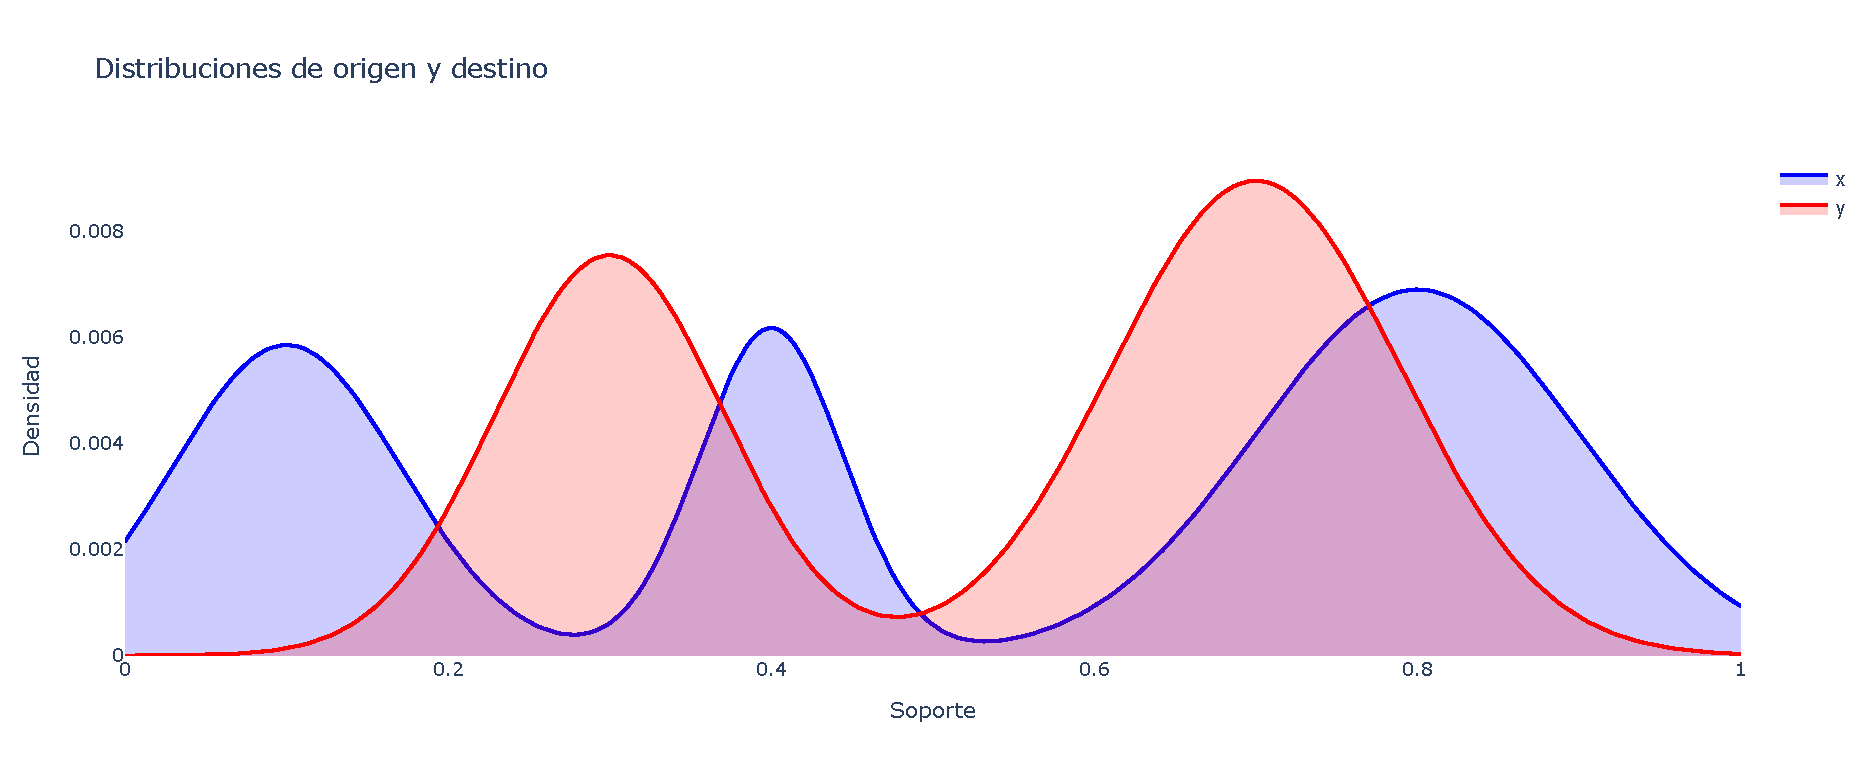
\includegraphics[width=0.9\textwidth]{images/ot/kantorovich_continuous_density}

	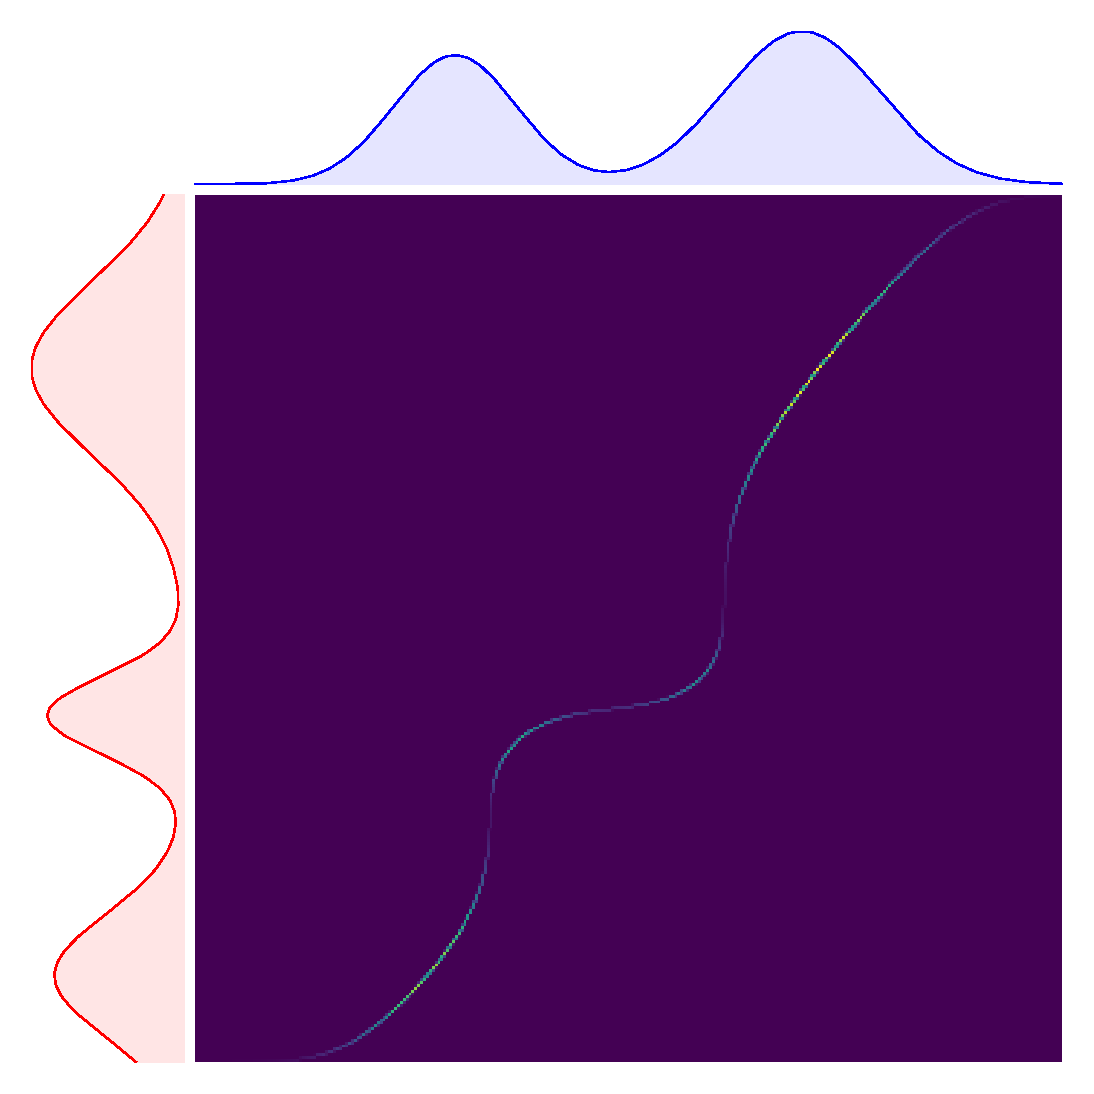
\includegraphics[width=0.4\textwidth]{images/ot/kantorovich_continuous_solution}
	\caption{(Arriba) gráficos de funciones de densidad asociadas a las medidas $\mu$ y $\nu$ respectivamente. (Abajo) solución para el problema de Kantorovich entre ambas medidas. Se observa como toda la masa de $\pi^*$ se concentra en una curva, la cual corresponde al gráfico del mapa de Monge para este mismo problema (ver \autoref{teo:brenier}). El código de esta simulación se encuentra en el archivo \texttt{kantorovich.ipynb}.}
	\label{fig:ot/kantorovich_continuous_example}
\end{figure}

\insertimage{ot/optimal_coupling1}{0.8}{Plan de Kantorovich para distintos pares de medidas $\alpha$ y $\beta$. (Arriba) las flechas indican cómo se debe repartir la masa de $\alpha$ en $\beta$ para el transporte óptimo en el sentido de Kantorovich. En el sentido de Monge, solo el 1º caso tiene solución ya que los otros casos requieren división de masa. (Abajo) coupling óptimo del problema. Imagen obtenida desde \cite{peyré2020computational}.}

\insertimage{ot/optimal_coupling2}{0.5}{Solución para el problema de Kantorovich entre dos medidas $\alpha$ y $\beta$. (Izquierda) coupling óptimo entre dos medidas continuas, donde la intensidad del color negro en la curva indica la densidad de masa del \textit{coupling} óptimo $\pi$ en cada punto del plano $\xspace\times\yspace$. Notar que, en este caso, el plan de Kantorovich está soportado precisamente en el gráfico del mapa de Monge. (Derecha) plan de Kantorovich $\pi$ entre dos medidas discretas, donde el radio de cada círculo es proporcional a la masa asignada a cada átomo de $\xspace\times\yspace$. Imagen obtenida desde \cite{peyré2020computational}.}

Es importante notar que los planes de transporte $\pi\in\Pi(\mu,\nu)$ se interpretan, al igual que en el caso discreto, considerando que $\d\pi(x,y)$ es la cantidad infinitesimal de masa transferida desde $\d x$ hacia $\d y$. Es decir, para un volumen $A\in\borel{\xspace}$ en el espacio de origen y un volumen $B\in\borel{\yspace}$ en el espacio de llegada, la cantidad de masa transferida desde $A$ hacia $B$ es precisamente $\pi(A\times B)$. En particular, al igual que para el caso discreto, la medida producto $\mu\otimes\nu\in\Pi\parent{\mu,\nu}$ es el plan de transporte que envía cada porción $A\in\borel{\xspace}$ a todo el espacio de llegada $\yspace$, repartiendo su masa de forma proporcional a la distribución que asigna $\nu$ sobre los elementos de $\yspace$.

Cuando se plantea el problema de transporte óptimo sobre un espacio común $\xspace=\yspace\subset\R^d$ (como en el problema de transporte de tierra de la \autoref{fig:ot/earth_mover}), es usual trabajar con funcionales de costo $c:\xspace\times\yspace\to\R_+$ de la forma $c(x,y)=d(x-y)$, donde $d:\R^d\to\R$ una función convexa por lo que, en estos casos, el problema de Kantorovich general sigue siendo un problema de optimización convexo. Un caso importante es considerar a $d$ como una norma en $\R^d$ ya que bajo este funcional de costo, el problema de Kantorovich permite definir una métrica entre las medidas $\mu$ y $\nu$, denominada distancia de Wasserstein y estudiada en la \autoref{ot/dynamic/wasserstein}. En particular, a lo largo de este trabajo será usual considerar un costo cuadrático mediante $d(z)=\frac{1}{2}\norm{z}^2$.

Con respecto a la existencia de una solución, si bien el conjunto factible $\Pi(\mu,\nu)$ es siempre no vacío, es necesario agregar una hipótesis de regularidad sobre la función de costo para garantizar que el ínfimo efectivamente se alcanza en algún plan de transporte óptimo:

\begin{prop}
	Dadas dos medidas de probabilidad, $\mu\in\probmeasure{\xspace}$, $\nu\in\probmeasure{\yspace}$ sobre los conjuntos $\xspace=\R^n$ e $\yspace=\R^m$, si $c:\xspace\times\yspace\to\R$ es un funcional continuo, entonces el problema de Kantorovich continuo \eqref{eq:kantorovich_continuous} posee solución.
\end{prop}

Para demostrar esta propiedad es usual estudiar el problema dual continuo \eqref{eq:kantorovich_dual_continuous}, el cual suele ser más fácil de trabajar. Sin embargo, en \cite{villani2003topics} realizan una demostración bajo hipótesis más débiles haciendo uso de resultados de topología y teoría de la medida\footnote{El teorema de Prokhorov permite concluir que $\Pi(\mu,\nu)$ es compacto para la convergencia débil (ver \autoref{defn:measure_weak_convergence}), mientras que una semicontinuidad inferior para $c$ permite concluir que el funcional $\pi\mapsto \int c\d\pi$ es continuo bajo esta topología, concluyendo el resultado mediante el teorema de Weierstrass.}.

Con respecto a la relación entre el problema de Monge y el problema de Kantorovich, se tiene la misma desigualdad que en el caso discreto (ver \autoref{prop:monge_kantorovich_discrete_inequality}). Además, se precisará una condición suficiente para alcanzar la igualdad, la cual será útil en el \autoref{teo:brenier}:

\begin{prop}
	\label{prop:monge_kantorovich_ineq_continuous}
	Se tiene la siguiente desigualdad para los problemas de Monge y Kantorovich:

	\begin{equation*}
		\inf_{\pi \in \Pi(\mu,\nu)} \int_{\xspace\times\yspace} c(x, y) \d\pi(x, y) \leq
		\inf_{\feasible{T:\xspace\to\yspace}{T_\#\mu=\nu}}
		\int_{\xspace} c(x, T(x)) \d\mu(x).
	\end{equation*}

	Además, para que la igualdad se alcance basta que exista un plan de Kantorovich \textit{determinista} $\pi^*$ de la forma $\pi^* = (\operatorname{Id}\otimes T)_\#\mu$, donde $T:\xspace\to\yspace$ es algún un mapa de transporte. Más aún, este mapa de transporte $T$ es óptimo para el problema de Monge.
\end{prop}

En la proposición anterior, la igualdad $\pi^* = (\operatorname{Id}\otimes T)_\#\mu$ indica que el plan de transporte $\pi^*$ es la medida push-forward que induce $\mu$ en $\xspace\times\yspace$ a través de la función $x\in\xspace\mapsto (x,T(x))\in\xspace\times\yspace$ (ver \autoref{fig:ot/deterministic_plan}). Este plan de transporte se considera determinista debido a que no realiza división de masa. En efecto, por la propia definición de $\pi^*$, su soporte está contenido en el grafo del mapa de transporte $T$:

\begin{equation*}
	\supp{\pi^*}
	\subset \operatorname{gr}(T) := \{(x,T(x)) : x\in\xspace\}
	\subset \xspace\times\yspace.
\end{equation*}

Por lo que es posible recuperar un mapa de transporte (el mismo mapa $T$) a partir de $\pi^*$, lo cual no es posible para planes de transporte generales que no tienen esta propiedad de determinismo. En estos casos, se debe recurrir a otras técnicas como las proyecciones baricéntricas, las cuales son usadas en el \autoref{eot_sbp} y estudiadas en más detalle en \cite{peyré2020computational}.

En el caso particular $\xspace=\yspace\subset\R^d$, bajo algunas hipótesis adicionales, sí es posible encontrar planes de Kantorovich deterministas. Sin embargo, para obtener este resultado será necesario estudiar la formulación dual del problema de Kantorovich la cual será utilizada posteriormente, en su versión regularizada, para desarollar el algoritmo de Sinkhorn, el cual es el algoritmo por defecto para resolver el problema del puente de Schrödinger.

Para el estudio de planes de transporte deterministas, es útil que una medida conjunta de la forma $\pi = \parent{\operatorname{Id}\otimes T}_\#\mu$ se puede expresar equivalentemente como $\d\pi(x,y) = \d\mu(x)\delta_{y=T(x)}$, lo cual evidencia el determinismo de este tipo de planes de transporte: la masa transportada desde $x$ hacia $y$ (indicada por $\d\pi(x,y)$) es, o bien toda la masa $\d\mu(x)$ si $y=T(x)$, o bien cero. 

Por otra parte, en algunos casos es útil la siguiente propiedad: la pertenencia al conjunto de couplings $\Pi(\mu,\nu)$ se puede caracterizar mediante funciones test.

\begin{prop}[caracterización de couplings]
	Dadas dos medidas de probabilidad, $\mu\in\probmeasure{\xspace}$ y $\nu\in\probmeasure{\yspace}$, definidas sobre $\xspace=\R^n$ e $\yspace=\R^m$. Entonces, para $\pi\in\probmeasure{\mu,\nu}$ se cumple que $\pi\in\Pi(\mu,\nu)$ si y solo si

	\begin{equation*}
		\int_{\xspace\times\yspace} (\phi\oplus\psi)(x,y)\d\pi(x,y) =
		\int_\xspace \phi(x)\d\mu(x) + \int_\yspace \psi(y)\d\nu(y),
		\quad\forall (\phi,\psi)\in \lspace{1}{\xspace}\times \lspace{1}{\yspace},
	\end{equation*}

	donde $\phi\oplus\psi:\xspace\times\yspace\to\R$ es la suma tensorial: $(\phi\oplus\psi)(x,y):=\phi(x)+\psi(y)$.
\end{prop}

Por último, dado que los planes de transporte son elementos de $\probmeasure{\xspace\times\yspace}$, siempre se puede asociar una variable aleatoria conjunta $(x,y)\sim\pi$ a un plan de transporte $\pi\in\Pi(\mu,\nu)$, donde la primera marginal, $x$ tendrá distribución $\mu$, mientras que la segunda marginal, $y$, tendrá distribución $\nu$. Además, esta interpretación permite escribir el problema de Kantorovich como

\begin{equation*}
	\min_{\pi\in\Pi(\mu,\nu)} \E{(x,y)\sim\pi}{c(x,y)}.
\end{equation*}

\subsection{Formulación dual}
\label{ot/kantorovich/dual}

Dado que el problema de Kantorovich es un problema de minimización convexo (al menos su versión discreta \eqref{eq:kantorovich_discrete}), es natural preguntarse por su problema dual, el cual es un problema de maximización convexo. Como se verá a continuación, la formulación dual reduce significativamente la cantidad de incógnitas buscadas en el problema de optimización. Además, el hecho de trabajar con un problema primal convexo permitirá concluir que hay dualidad fuerte tanto en el caso discreto como en el caso continuo.

\subsubsection{Problema dual discreto}

Dado que el problema de Kantorovich discreto \eqref{eq:kantorovich_discrete} es un problema de programación lineal, su problema dual es otro problema de programación lineal cuya forma es conocida (ver, por ejemplo, \cite{boyd2004convex}):

\begin{prop}[dualidad fuerte para Kantorovich, caso discreto]
	\label{prop:duality_discrete}
	El problema dual del problema de Kantorovich discreto \eqref{eq:kantorovich_discrete} es:

	\begin{equation}
		\label{eq:kantorovich_dual_discrete}
		\sup_{\feasible{(\phi,\psi)\in\R^n\times\R^m} {\phi\oplus \psi \leq C}}
		\dotproduct{\phi}{a} + \dotproduct{\psi}{b} = \sum_{i=1}^n \phi_i a_i + \sum_{j=1}^m \psi_j b_j ,
	\end{equation}

	donde la restricción $\phi\oplus \psi \leq C$ indica que $\phi_i+\psi_j \leq C_{ij}, \, \forall i\in\{1,\ldots,n\}, \, \forall j\in\{1,\ldots,m\}$. Además, hay dualidad fuerte:

	\begin{equation}
		\label{eq:kantorovich_strong_duality_discrete}
		\inf_{P\in \Pi_d(\mu,\nu)} \dotproduct{C}{P}_F
		= \sup_{\feasible{(\phi,\psi)\in\R^n\times\R^m}{\phi\oplus \psi \leq C}}
		\dotproduct{\phi}{a} + \dotproduct{\psi}{b}.
	\end{equation}

	Por otra parte, a un par de vectores duales óptimos, $(\phi^*,\psi^*)\in\R^n\times\R^m$, se les denomina \textit{potenciales de Kantorovich}.
\end{prop}

Notar que en esta proposición, la notación $\phi\oplus\psi\in\matrixspace{n,m}{\R}$ representa la suma tensorial entre $\phi$ y $\psi$: $\parent{\phi\oplus\psi}_{ij}=\phi_i+\psi_j$ o, equivalentemente, $\phi\oplus\psi = \phi\1_m^\top + \1_n \psi^\top$. Por otra parte, la propiedad de dualidad permite caracterizar las soluciones primales-duales mediante las condiciones de Karush-Kuhn-Tucker (ver \cite{boyd2004convex}). Más precisamente, se puede concluir el siguiente resultado:

\begin{cor}
	Sea $(\phi^*,\psi^*)\in\R^n\times\R^m$ un par de potenciales de Kantorovich asociados al problema dual \eqref{eq:kantorovich_dual_discrete}. Entonces, cualquier solución $P^*\in\Pi_d(\mu,\nu)$ para el problema primal \eqref{eq:kantorovich_discrete} tiene su soporte en las coordenadas donde se cumple la restricción dual con igualdad:

	\begin{equation*}
		\{(i,j):\,P_{ij}^*>0\}
		\subset \{(i,j):\, \phi^*_i + \psi^*_j = C_{ij}\},
		\subset \{1,\ldots,n\}\times\{1,\ldots,m\}.
	\end{equation*}

\end{cor}

\begin{proof}
	Esta propiedad es consecuencia directa de la propiedad de holgura complementaria. En efecto, la restricción dual asociada a la variable primal $P_{ij}$ es $\phi_i + \psi_j - C_{ij}\leq 0$, por lo que la propiedad de holgura complementaria indica que $P_{ij}\parent{\phi_i + \psi_j - C_{ij}} = 0$. En particular, si $P_{ij}>0$ entonces $\phi_i + \psi_j - C_{ij} = 0$.
\end{proof}

Una ventaja importante que se obtiene al usar la formulación dual se observa al momento de intentar resolver numéricamente el problema de Kantorovich. En efecto, para resolver el problema de Kantorovich discreto \eqref{eq:kantorovich_discrete} es necesario encontrar una matriz $P\in\Pi_d(\mu,\nu)$ ($n\cdot m$ incógnitas), mientras que al usar la formulación discreta dual \eqref{eq:kantorovich_dual_discrete} solo es necesario encontrar dos vectores $(\phi,\psi)\in\R^n\times\R^m$ ($n+m$ incógnitas). Sin embargo, una solución dual $(\phi^*,\psi^*)$ no permite obtener directamente una solución primal como sí ocurre en la formulación regularizada del problema de Kantorovich (ver \autoref{prop:eot_dual_discrete}) ya que no es posible \textit{despejar} una solución primal desde la formulación dual.

Por otra parte, una forma usual de interpretar el problema de Kantorovich discreto dual es mediante el problema de transporte desde yacimientos hacia fábricas. Para esto, se puede considerar que el dueño de los yacimientos decide contratar una empresa externa que realice el servicio de transporte de la materia prima, pagando una cantidad $\phi_i$ por cargar una unidad de materia prima desde el yacimiento $i$, y una cantidad $\psi_j$ por descargar una unidad de materia prima en la fábrica $j$, sin importar la forma en cómo se distribuyen los recursos de acuerdo a un plan de transporte. Desde el punto de vista de la empresa externa, esta buscará vectores de cobro $\phi\in\R^n$ y $\psi\in\R^m$ que maximicen su ganancia y considerando que $\phi_i+\psi_j\leq C_{ij}$ ya que, de lo contrario, el dueño de los yacimientos no tendrá motivos para realizar el transporte con esta empresa. La dualidad fuerte entregada en \eqref{eq:kantorovich_strong_duality_discrete} afirma que la empresa externa puede encontrar vectores de cobro $(\phi^*,\psi^*)$ tales que su ganancia sea igual al costo de transporte original que hubiese pagado el dueño de los yacimientos si realizara el transporte sin la empresa externa.

\subsubsection{Problema dual continuo}

En el caso continuo, se tiene un resultado análogo al presentado en la \autoref{prop:duality_discrete}. Sin embargo, al igual que para la formulación primal continua, hay que agregar hipótesis de regularidad extras sobre la función de costo para poder garantizar la dualidad fuerte.

\begin{teo}[dualidad fuerte para Kantorovich, caso continuo]
	\label{teo:kantorovich_dual_continuous}
	Si $c:\xspace\times\yspace\to\R$ es un funcional de costo continuo y acotado inferiormente, entonces, el problema dual del problema de Kantorovich continuo \eqref
	{eq:kantorovich_continuous} es:

	\begin{equation}
		\label{eq:kantorovich_dual_continuous}
		\sup_{\feasible{(\phi,\psi)\in \lspace{1}{\xspace}\times\lspace{1}{\yspace}}{\phi\oplus\psi\leq c}}
		\int_{\xspace} \phi(x) \d\mu(x) + \int_{\yspace} \psi(y) \d\nu(y) ,
	\end{equation}

	donde la restricción $\phi\oplus\psi\leq c$ indica que $(\phi\oplus\psi)(x,y):=\phi(x)+\psi(y)\leq c(x,y),\,\forall x\in\xspace,\,\forall y\in\yspace$\footnote{En rigor, esta igualdad es casi seguramente. Sin embargo, se puede demostrar que los potenciales se pueden elegir continuos, recuperando la igualdad puntual.}.

	Además, hay dualidad fuerte:

	\begin{equation*}
		\inf_{\pi\in\Pi(\mu,\nu)} \int_{\xspace\times\yspace} c(x, y) \d\pi(x, y)
		= \sup_{\feasible{(\phi,\psi)\in \lspace{1}{\xspace}\times\lspace{1}{\yspace}}{\phi\oplus\psi\leq c}}
		\int_{\xspace} \phi(x) \d\mu(x) + \int_{\yspace} \psi(y) \d\nu(y) .
	\end{equation*}

	Por otra parte, a un par de funcionales duales óptimos, $(\phi^*,\psi^*)\in\lspace{1}{\xspace}\times\lspace{1}{\yspace}$, se les denomina \textit{potenciales de Kantorovich}.
\end{teo}

Una demostración de esta propiedad se puede encontrar en \cite{villani2003topics}, donde además muestran que los potenciales de Kantorovich $(\phi^*,\psi^*)\in \lspace{1}{\xspace}\times\lspace{1}{\yspace}$ se pueden elegir continuos y acotados, pudiendo optimizar el problema dual sobre $\continuousb{\xspace}\times\continuousb{\yspace}\subset\lspace{1}{\xspace}\times\lspace{1}{\yspace}$. Esto es posible debido a que las funciones en $\continuousb{\R^d}$ son capaces de aproximar suficientemente bien a las funciones en $L^1(\R^d)$\footnote{Más precisamente, dada una medida de probabilidad $\mu\in\probmeasure{\R^d}$, el conjunto $\continuousb{\R^d}\subset L^1(\R^d,\mu)$ es denso en $L^1(\R^d,\mu)$: para cualquier función $f\in L^1(\R^d,\mu)$ y error $\epsilon>0$, existe una función $g\in\continuousb{\R^d}$ tal que $\int_{\R^d} |f-g| \d\mu<\epsilon$.}. De todos modos, por simplicidad, se seguirán considerando que los potenciales de Kantorovich son funciones genéricas en $\lspace{1}{\xspace}$ y $\lspace{1}{\yspace}$ respectivamente.

Al igual que para el caso discreto, el soporte para el plan de transporte óptimo está contenido en el subconjunto que activa la desigualdad dual en \eqref{eq:kantorovich_dual_continuous}:

\begin{cor}
	\label{cor:supp_slackness}
	Sea $(\phi^*,\psi^*)\in \lspace{1}{\xspace}\times\lspace{1}{\yspace}$ un par de potenciales de Kantorovich asociados al problema dual \eqref{eq:kantorovich_dual_continuous}. Entonces, cualquier solución $\pi^*\in\Pi(\mu,\nu)$ para el problema primal \eqref{eq:kantorovich_continuous} tiene su soporte en un subconjunto específico de $\xspace\times\yspace$:

	\begin{equation*}
		\supp{\pi^*}
		\subset \{(x,y)\in\xspace\times\yspace:\, \phi^*(x) + \psi^*(y) = c(x,y)\}
	\end{equation*}.
\end{cor}

El problema dual permitirá demostrar que el problema de Kantorovich es equivalente (en el sentido que lo indicará el \autoref{teo:brenier}) al problema de Monge en el caso particular $\xspace=\yspace\subset\R^d$ cuando se considera un costo cuadrático, el cual es el escenario más importante debido a su conexión con el problema de Schrödinger con prior browniano en el \autoref{eot_sbp}. Para mostrar este resultado (conocido como teorema de Brenier), se vuelve necesario revisar algunos conceptos de análisis convexo:

\begin{defn}[subdiferencial]
	Dada una función convexa $f:\R^d\to\R$, su \textit{subdiferencial} $\partial f$ es la función (multivaluada) que asigna a cada $x\in\R^d$ un conjunto de subgradientes:

	\begin{equation}
		\label{eq:subdiferential}
		\partial f(x) := \{y\in\R^d\,:\,f(z)\geq \tilde{f}_y(z) := f(x) + \dotproduct{y}{z-x},\,\forall z\in\R^d\}.
	\end{equation}

\end{defn}

Este concepto permite generalizar el concepto de gradiente a funciones convexas que no necesariamente son diferenciables en todo su dominio. En efecto, la desigualdad en \eqref{eq:subdiferential} indica que la recta tangente $\tilde{f}_y$ (cuya pendiente es $y\in\partial f(x)$) está siempre por debajo del gráfico de $f$, lo cual es una propiedad que caracteriza a las funciones convexas diferenciables. En la \autoref{fig:ot/subdifferential} se puede ver el subdiferencial de una función no diferenciable. Se puede probar lo siguiente (ver, por ejemplo, \cite{villani2003topics}):


\begin{prop}
	Sea $f:\R^d\to\R$ una función diferenciable en $x\in\R^d$. Entonces, $\partial f(x)=\{\nabla f(x)\}$.
\end{prop}

Este resultado es el que permitirá posteriormente caracterizar el mapa de Monge $T:\xspace\to\yspace$ como el gradiente de una función convexa en el \autoref{teo:brenier}.

\insertimage{ot/subdifferential}{0.5}{La función $f$ no es diferenciable en $x=1$, por lo que su conjunto de subgradientes no será un único punto. Las rectas $g_i,\,i\in\{1,2,3,4\}$ son tangentes a $f$ en $(1,1)$, por lo que sus pendientes corresponden a subgradientes de $f$. Esta imagen se encuentra en el archivo \texttt{subdifferential.ipynb}.}

Por otra parte, el concepto de transformada de Legendre permitirá reescribir la condición de factibilidad dual $\phi\oplus\psi\leq c$ utilizando el concepto de subdiferencial:

\begin{defn}[transformada de Legendre]
	\label{defn:legendre}
	Dada una función $f:\R^d\to\R$, su \textit{transformada de Legendre}\footnote{En la literatura es usual usar la notación $f^*$ en vez de $f_*$. Aquí se preferirá la segunda notación para no confundir con la notación usada para soluciones óptimas.} es otra función $f_*:\R^d\to\R$ definida por:

	\begin{equation*}
		f_*(y) := \sup_{x\in\R^d} \dotproduct{x}{y} - f(x) .
	\end{equation*}
\end{defn}

La importancia de la transformada de Legendre, en este caso, es que permite caracterizar completamente el subdiferencial de una función convexa. En efecto, se tiene el siguiente resultado:

\begin{prop}
	\label{prop:subdiff_legendre}
	Dada una función convexa y continua $f:\R^d\to\R$, se tiene que $\forall x,y\in\R^d$,

	\begin{equation*}
		y\in\partial f(x) \Leftrightarrow f(x) + f_*(y) = \dotproduct{x}{y}.
	\end{equation*}
\end{prop}

Con estos resultados auxiliares, se puede enunciar y demostrar el teorema de Brenier, el cual es un resultado clave que permite obtener soluciones del problema de Monge a partir del problema de Kantorovich, y viceversa (ver \autoref{fig:ot/kantorovich_continuous_example}):

\begin{teo}[Brenier]
	\label{teo:brenier}
	Sean $\mu\in\probmeasure{\xspace}$ y $\nu\in\probmeasure{\yspace}$ medidas de probabilidad en $\xspace=\yspace=\R^d$ con segundo momento finito\footnote{Los momentos de una medida de probabilidad $\mu\in\probmeasure{\R^d}$ son los momentos de una variable aleatoria cuya ley es $\mu$.}:

	\begin{equation*}
		\int_{\xspace} \norm{x}^2 \d\mu(x)<\infty,
		\qquad
		\int_{\yspace} \norm{y}^2 \d\nu(y)<\infty .
	\end{equation*}

	Si $\mu$ posee una función de densidad asociada\footnote{Esta hipótesis se puede relajar a que $\mu\in\probmeasure{\xspace}$ no le entregue masa a conjuntos medibles con dimensión de Hausdorff-Besicovitch menor que $d$.}, entonces existe una única solución $\pi^*\in\Pi(\mu,\nu)$ para el problema de Kantorovich \eqref{eq:kantorovich_continuous} con costo cuadrático, $c(x,y)=\frac{1}{2}\norm{x-y}^2$. Además, esta solución es determinista (en el sentido que lo indica la \autoref{prop:monge_kantorovich_ineq_continuous}) y de la forma

	\begin{equation*}
		\pi^* = \parent{\operatorname{Id}\otimes \nabla f}_\#\mu ,
	\end{equation*}

	para alguna función convexa $f:\R^d\to\R$.
\end{teo}

\begin{proof}
	Para empezar, notar que la función objetivo en \eqref{eq:kantorovich_continuous} con $c(x,y)=\frac{1}{2}\norm{x-y}^2$ se puede descomponer como $c(x,y)=\frac{1}{2}\parent{\norm{x}^2+\norm{y}^2}+\dotproduct{x}{y}$, por lo tanto:

	\begin{align*}
		\int_{\xspace\times\yspace} c(x,y) \d\pi(x,y) & = \frac{1}{2}\int_{\xspace\times\yspace} \parent{\norm{x}^2 + \norm{y}^2} \d\pi(x,y) - \int_{\xspace\times\yspace} \dotproduct{x}{y} \d\pi(x,y)                                 \\
		                                        & = \underbrace{\frac{1}{2}\parent{\int_{\xspace} \norm{x}^2 \d\mu(x) + \int_{\yspace} \norm{y}^2 \d\nu(y)}}_{<\infty} - \int_{\xspace\times\yspace} \dotproduct{x}{y} \d\pi(x,y).
	\end{align*}

	Donde el primer sumando (finito) es constante con respecto a $\pi$, por lo que es suficiente resolver el siguiente problema de optimización:

	\begin{equation*}
		\sup_{\pi\in\Pi(\mu,\nu)} \int_{\xspace\times\yspace} \dotproduct{x}{y} \d\pi(x,y).
	\end{equation*}

	Análogo a lo obtenido en el \autoref{teo:kantorovich_dual_continuous} (y recordando que los potenciales de Kantorovich se podían elegir continuos), el dual de este nuevo problema es:

	\begin{equation}
		\label{eq:brenier_dual}
		\inf_{\feasible{(f,g)\in \continuousb{\xspace}\times\continuousb{\yspace}}{f\oplus g \geq \dotproduct{\cdot}{\cdot}}}
		\int_{\xspace} f(x) \d\mu(x) + \int_{\yspace} g(y) \d\nu(y).
	\end{equation}

	Por otra parte, si se fija la primera variable dual, $f\in \continuousb{\xspace}$, la restricción $f\oplus g \geq \dotproduct{\cdot}{\cdot}$ se puede reescribir de la siguiente forma:

	\begin{alignat*}{3}
		& f(x)+g(y) \geq \dotproduct{x}{y}, &\forall x\in\xspace,y\in\yspace                                           \\
		 & \iff g(y) \geq \dotproduct{x}{y} - f(x), &\forall x\in\xspace,y\in\yspace                                  \\
		 & \iff g(y) \geq \underbrace{\sup_{x\in\xspace} \dotproduct{x}{y} - f(x)}_{f_*(y)}, &\forall y\in\yspace .
	\end{alignat*}

	Por lo tanto, para minimizar el funcional $g \mapsto \int_{\yspace} g(y) \d\nu(y)$ (recordar que $f$ está fija) respetando la restricción $f\oplus g \geq \dotproduct{\cdot}{\cdot}$ basta tomar $g=f_*$. En consecuencia, el problema \eqref{eq:brenier_dual} se puede reescribir de forma irrestricta mediante la siguiente formulación semidual:

	\begin{equation*}
		\inf_{f\in \continuousb{\xspace}}
		\int_{\xspace} f(x) \d\mu(x) + \int_{\yspace} f_*(y) \d\nu(y) .
	\end{equation*}

	Del mismo modo, fijando ahora la segunda variable dual, $g=f_*$, se muestra que la restricción $f\oplus g \geq \dotproduct{\cdot}{\cdot}$ es equivalente a la restricción $f(x) \geq f_{**}(x) = \sup_{y\in\yspace} \dotproduct{x}{y} - f_*(x),\,\forall x\in\xspace$, por lo que, nuevamente, se puede elegir a $f_{**}$ como el primer potencial para minimizar ahora la primera integral.

	En consecuencia, dado que la transformada de Legendre define una función convexa, se puede restringir la búsqueda a potenciales $f\in \continuousb{\xspace}$ convexos:

	\begin{equation*}
		\inf_{f\in \continuousb{\xspace}\text{ convexa}}
		\int_{\xspace} f(x) \d\mu(x) + \int_{\yspace} f_*(y) \d\nu(y).
	\end{equation*}

	Por otra parte, si $f^*$ es una variable dual óptima, por la condición de holgura complementaria (análogo a lo realizado en el \autoref{cor:supp_slackness}):

	\begin{equation*}
		\supp{\pi^*}
		\subset \{(x,y)\in\xspace\times\yspace:\, f^*(x) + f_*^*(y) = \dotproduct{x}{y}\}.
	\end{equation*}

	Notar que, gracias a la \autoref{prop:subdiff_legendre}, la igualdad $f^*(x) + f_*^*(y) = \dotproduct{x}{y}$ se alcanza si y solo si $y\in\partial f^*(x)$. Además, como la variable dual $f^*$ es convexa y $\mu$ tiene función de densidad, resulta ser que $f^*$ es diferenciable en $\xspace$\footnote{Esto es consecuencia del teorema de Rademacher.}. De esta forma, $\partial f(x) = \{\nabla f(x)\}$, y así

	\begin{equation*}
		\supp{\pi^*}
		\subset \{(x,\nabla f^*(x)):\,x\in\xspace\} \subset \xspace\times\yspace .
	\end{equation*}

	Por lo que $\pi^*$ es una medida producto soportada en el grafo de la función $\nabla f^*$ y así, es un plan de transporte determinista con $\pi^*=(\operatorname{Id}\otimes\nabla f^*)_\# \mu$.
\end{proof}

Una consecuencia directa de este teorema es que permite obtener resultados de existencia y unicidad para el problema de Monge con costo cuadrático:

\begin{cor}
	Bajo las hipótesis del \autoref{teo:brenier}, el mapa de transporte $T=\nabla f$ es la única solución del problema de Monge con funcional de costo $c(x,y)=\frac{1}{2}\norm{x-y}^2$.
\end{cor}

\begin{proof}
	Notar que, por definición de $\pi^* = \parent{\operatorname{Id}\otimes \nabla f}_\#\mu$, el mapa $x\in\xspace \mapsto \nabla f(x)\in\yspace$ cumple la propiedad $(\nabla f)_\#\mu=\nu$, por lo que $T=\nabla f$ es efectivamente un mapa de transporte. Por otra parte, dado que $\pi^*$ es un plan de transporte determinista y óptimo, por la \autoref{prop:monge_kantorovich_ineq_continuous} se concluye que $\nabla f$ es solución del problema de Monge. Además, como el \autoref{teo:brenier} garantiza unicidad para $\pi^*$, se obtiene la unicidad de la solución para el problema de Monge.
\end{proof}

\subsection{Casos particulares en \texorpdfstring{$\R^d$}{Rd}}
\label{ot/kantorovich/rd}

Si bien los problemas de transporte óptimo son complejos de analizar en general, existen algunos casos particulares en donde la solución se puede caracterizar fácilmente.

\subsubsection{Transporte óptimo unidimensional}

En el caso unidimensional $\xspace=\yspace=\R$, la solución para los problemas de transporte óptimo se pueden definir haciendo uso de la función de distribución acumulada y su respectiva inversa, la función cuantil. La primera de estas funciones tiene la siguiente definición:

\begin{defn}[función de distribución acumulada]

	Dada una medida de probabilidad $\mu\in\probmeasure{\R}$, su \textit{función de distribución acumulada} $F_\mu:\R\to[0,1]$ se define como:

	\begin{equation*}
		F_\mu(x) := \int_{-\infty}^x \d\mu(s) = \int_{-\infty}^x p(s)\d s,
	\end{equation*}

	donde la última igualdad solo tiene sentido si $\mu$ posee una función de densidad $p$.

\end{defn}

Es importante recordar que la función de distribución acumulada $F_\mu$ identifica totalmente a la medida de probabilidad $\mu$\footnote{Dado que $\mu\parent{(a, b]} = F_\mu(b) - F_\mu(a)$, se tiene que $F_\mu$ determina el valor de $\mu$ en una semi-álgebra de $\R$, por lo cual la extensión de Carathéodory es única.}. El siguiente teorema entrega la solución para el problema de Kantorovich entre dos medidas de probabilidad en $\R$:

\begin{teo}
	\label{teo:kantorovich_r}
	Sean $\mu\in\probmeasure{\xspace}$ y $\nu\in\probmeasure{\yspace}$ dos medidas de probabilidad en $\xspace=\yspace=\R$ con funciones de distribución acumulada $F_\mu$ y $F_\nu$ respectivamente. Entonces, el plan de transporte óptimo, $\pi^*\in\Pi(\mu,\nu)$, para el problema de Kantorovich entre $\mu$ y $\nu$ con función de costo $c(x,y)=|x-y|$ tiene la siguiente función de distribución acumulada:

	\begin{equation*}
		F_{\pi^*}(x,y) = \inf \{F_\mu(x),F_\nu(y)\} .
	\end{equation*}

	Además, el valor óptimo del problema de Kantorovich es la distancia $\lspace{1}{\R}$ entre las funciones de distribución acumulada de $\mu$ y $\nu$:

	\begin{equation*}
		\inf_{\pi \in \Pi(\mu,\nu)} \int_{\xspace\times\yspace} |x-y| \d\pi(x, y)
		= \norm{F_\mu-F_\nu}_{L^1(\xspace)}
		:= \int_{-\infty}^\infty \left|F_\mu(z)-F_\nu(z)\right| \d z .
	\end{equation*}
\end{teo}

Para extender el resultado a funcionales de costo de la forma $c(x,y)=|x-y|^p$ será necesario introducir la función cuantil: 

\begin{defn}[función cuantil]
	Dada una medida de probabilidad $\mu\in\probmeasure{\R}$ con función de distribución acumulada $F_\mu$, se define la \textit{función cuantil} de $\mu$, $Q_\mu:[0,1]\to\R$, como:

	\begin{equation*}
		Q_\mu(z) := \inf \{x\in\R\,:\, F_\mu(x)\geq z\}.
	\end{equation*}
\end{defn}

Esta función actúa como función inversa de la función de distribución acumulada ya que si $F_\mu$ es además estrictamente creciente se obtiene que $Q_\mu(z) = F_\mu^{-1}(z)$, mientras que en los casos donde no hay invertibilidad, se tiene que $F_\mu^{-1}(F_\mu(x)) \geq x$ y $F(F_\mu^{-1}(z)) \geq z$, por lo que se suele decir que es su inversa por la izquierda.

Con esta definición, se tiene el siguiente resultado:

\begin{teo}
	Sean $\mu\in\probmeasure{\xspace}$ y $\nu\in\probmeasure{\yspace}$ dos medidas de probabilidad en $\xspace=\yspace=\R$ con funciones de distribución acumulada $F_\mu$ y $F_\nu$ respectivamente. Entonces, para el funcional de costo $c(x,y)=|x-y|^p,\,p\geq 1$, se tiene que un mapa de transporte óptimo para el problema de Monge \eqref{eq:monge_continuous} es

	\begin{equation*}
		T(x) = Q_\nu\parent{F_\mu(x)}.
	\end{equation*}

	Mientras que el valor óptimo para el problema de Kantorovich es la distancia $L^1$ de sus funciones cuantil:

	\begin{equation*}
		\norm{Q_\mu-Q_\nu}_{L^1([0,1])}:=\int_0^1 |Q_\mu(z) - Q_\nu(z)|^p \d z .
	\end{equation*}
\end{teo}

Las demostraciones de estos resultados se pueden encontrar en \cite{Thorpe2018}.

\subsubsection{Transporte óptimo entre distribuciones gaussianas}

Otro caso donde se puede encontrar una solución de forma cerrada ocurre cuando se consideran las leyes de dos distribuciones gaussianas con un funcional de costo cuadrático:

\begin{teo}
	\label{teo:frechet_gaussian}
	Dadas dos variables aleatorias gaussianas, $x\sim\gaussian{\mu_1}{\Sigma_1}$ e $y\sim \gaussian{\mu_2}{\Sigma_2}$, si se considera $\mu=\ley{x}$ y $\nu=\ley{y}$ las respectivas medidas asociadas a $x$ e $y$ respectivamente\footnote{Para una variable aleatoria $x\sim p(x)$ (con $p:\xspace\to\R_+$ su función de densidad), su ley es la medida $\mu_x(A)=\int_A p(x)\d x$}, entonces, el valor óptimo para el problema de Kantorovich \eqref{eq:kantorovich_continuous} entre $\mu$ y $\nu$ con $c(x,y)=\norm{x-y}^2$ es

	\begin{equation*}
		\norm{\mu_1-\mu_2}_2^2 + \trace{\Sigma_1+\Sigma_2 - 2\left(\Sigma_1^\frac{1}{2}\Sigma_2\Sigma_1^\frac{1}{2}\right)^\frac{1}{2}} .
	\end{equation*}

	Además, el mapa de Monge asociado $T:\R^d\to\R^d$ viene dado por

	\begin{equation*}
		T(x) = \mu_2 + A(x - \mu_1),
		\quad\text{donde}\quad
		A = \Sigma_1^{-1/2}\left(\Sigma_1^{1/2} \Sigma_2 \Sigma_1^{1/2}\right)^{1/2}\Sigma_1^{-1/2} .
	\end{equation*}
\end{teo}

\insertimage{ot/gaussian_interpolation}{1}{Interpolación entre dos curvas gaussianas utilizando la solución cerrada del \autoref{teo:frechet_gaussian}. El código de esta simulación se encuentra en el archivo \texttt{distr\_interpolation.ipynb}.}

La demostración de esta propiedad se puede encontrar en \cite{peyré2020computational}. Por otro lado, en la \autoref{fig:ot/gaussian_interpolation} se observa el problema de transporte entre dos gaussianas de una forma dinámica, donde se ve la \textit{trayectoria} que la distribución debe seguir durante el transporte. Esto será estudiado en la \autoref{ot/dynamic}. 

El \autoref{teo:frechet_gaussian} entrega de forma explícita el mapa de Monge para el problema de transporte óptimo, el cual se sabe que existe gracias al \autoref{teo:brenier}. Además, es importante notar que $\Sigma_1$ y $\Sigma_2$ son matrices de covarianzas, por lo que deben ser simétricas y definidas positivas (asumiendo que $x$ e $y$ son variables aleatorias gaussianas no degeneradas). De este modo, la descomposición de Cholesky garantiza que sus raíces cuadradas están bien definidas y, por lo tanto, la matriz $A$ está bien definida.

Por otra parte, la matriz $A$ puede ser interpretada como una transformación lineal. De esta forma, el operador $T$ es un operador afín que primero traslada las masas de $x\sim \gaussian{\mu_1}{\Sigma_1}$ al origen mediante $x-\mu_1$ y luego aplica la transformación lineal. Finalmente, $T$ realiza una traslación al centro de $\gaussian{\mu_2}{\Sigma_2}$.

La transformación $x\mapsto Ax$ busca deformar la distribución $x\sim \gaussian{\mu_1}{\Sigma_1}$ para hacerla similar a la distribución $\gaussian{\mu_2}{\Sigma_2}$. Esto se vuelve evidente cuando se considera $d=1$ ya que, en ese caso, $A=\frac{\sigma_2}{\sigma_1} \in\mathbb{R}_+$ es la raiz cuadrada del ratio entre ambas varianzas.

Por último, es importante destacar que el valor óptimo para el problema de Kantorovich entre gaussianas es utilizado en la métrica FID al momento de evaluar algunos modelos generativos como los modelos de difusión (ver, por ejemplo, \cite{betzalel2022studyevaluationgenerativemodels}).

\subsubsection{Mapa de Monge a partir de un potencial de Kantorovich}

En la demostración del \autoref{teo:brenier} se utilizó la transformada de Legendre (\autoref{defn:legendre}) para reformular el problema dual (restringido) en un problema irrestricto, limitado únicamente a buscar sobre un tipo particular de funciones. En este apartado se extenderá esta idea al problema de Kantorovich con funcionales arbitrarios. Para un estudio más detallado, ver \cite{villani2003topics}.

En el problema dual \eqref{eq:kantorovich_dual_continuous}, los potenciales admisibles $(\phi,\psi)\in \lspace{1}{\xspace}\times\lspace{1}{\yspace}$ deben cumplir la restricción $\phi\oplus\psi\leq c$. Con esto, repitiendo la idea de la demostración del \autoref{teo:brenier}, si se fija el primer potencial $\phi\in\lspace{1}{\xspace}$, el segundo potencial $\psi\in \lspace{1}{\yspace}$ debe ser tal que

\begin{equation*}
	\psi(y) \leq c(x,y) - \phi(x), \quad \forall x\in\xspace,\,y\in\yspace
	\iff
	\psi(y) \leq \inf_{x\in\xspace} c(x,y) - \phi(x) .
\end{equation*}

Por lo que se puede elegir el segundo potencial como la función $\phi^c(y) = \inf_{x\in\xspace} c(x,y) - \phi(x)$ para maximizar la función objetivo cuando el primer potencial está fijo. Considerando ahora este nuevo potencial $\phi^c\in \lspace{1}{\yspace}$ como fijo, se puede realizar un procedimiento análogo para actualizar el primer potencial:

\begin{equation*}
	\phi(x) \leq c(x,y) - \phi^c(y), \quad \forall x\in\xspace,\,y\in\yspace
	\iff
	\phi(x) \leq \inf_{y\in\yspace} c(x,y) - \phi^c(y) .
\end{equation*}

Por lo que se puede actualizar el primer potencial a la función $\phi^{c\bar c}(x) := \inf_{y\in\yspace} c(x,y) - \phi^c(y)$ para maximizar la función objetivo cuando el segundo potencial está fijo. Este procedimiento motiva las siguientes definiciones, las cuales se pueden considerar como una generalización de la transformada de Legendre:

\begin{defn}[$c$-transformadas y concavidad]
	\label{defn:c_transform}
	Sean $f:\xspace\to\R$ y $g:\yspace\to \R$ funciones arbitrarias. Dado un funcional $c:\xspace\times\yspace\to\R$ acotado, se definen las siguientes transformaciones:

	\begin{itemize}
		\item \textit{$c$-transformada}  de $f$: función $f^c:\yspace\to\R$ definida como $f^c(y) := \inf\limits_{x\in\xspace} c(x,y) - f(x)$.

		\item \textit{$\bar c$-transformada}  de $g$: función $g^{\bar c}:\xspace\to\R$ definida como $g^{\bar c}(x) := \inf\limits_{y\in\yspace} c(x,y) - g(y)$.
	\end{itemize}

	Por otra parte, una función $f:\xspace\to\R$ se dirá $c$-cóncava si existe una función $g:\yspace\to\R$ tal que $f=g^{\bar c}$. Análogamente, una función $g:\yspace\to\R$ se dirá $\bar c$-cóncava si existe una función $f:\xspace\to\R$ tal que $g=f^c$.
\end{defn}

Notar que la única diferencia entre la $c$-transformada y la $\bar c$-transformada es la variable sobre la que actúa el funcional $c$. Por lo tanto, si $c$ es simétrico (i.e., $c(x,y)=c(y,x)$), ambas transformaciones son iguales.

Con estas definiciones, el procedimiento descrito anteriormente comienza con un primer potencial arbitrario, $\phi\in \lspace{1}{\xspace}$, y se va actualizando alternadamente el otro potencial de tal forma que en cada actualización el valor del funcional de optimización dual en \eqref{eq:kantorovich_dual_continuous} no empeora (y, eventualmente, mejora). Por lo tanto, la cadena de actualizaciones de potenciales es la siguiente:

\begin{equation}
	\label{eq:c_concave_actualization}
	(\phi,\phi^c) \to (\phi^{c\bar c}, \phi^c) \to (\phi^{c\bar c}, \phi^{c\bar c c}) .
\end{equation}

Si bien se podrían realizar estas iteraciones indefinidamente, se puede demostrar que $\phi^{c\bar c c} = \phi^c$, por lo que la tercera actualización, $(\phi^{c\bar c}, \phi^{c\bar c c})$, es equivalente a $(\phi^{c\bar c}, \phi^c)$, lo cual corresponde a la segunda iteración. Por lo tanto, este procedimiento no permite mejorar la función objetivo más allá de dos iteraciones. De todos modos, este método sugiere que basta encontrar un único potencial $\phi\in \lspace{1}{\xspace}$ para el problema dual \eqref{eq:kantorovich_dual_continuous}. Observando que $f=\phi^{c\bar c}$ en \eqref{eq:c_concave_actualization} es una función $c$-cóncava, se puede probar el siguiente resultado:

\begin{teo}[formulación dual mediante $c$-transformadas]
	\label{teo:dual_c_transform}
	Sea $c:\xspace\times\yspace\to\R$ un funcional de costo continuo y acotado con $\xspace\subset\R^n$ e $\yspace\subset\R^m$. Para dos medidas de probabilidad, $\mu\in\probmeasure{\xspace}$ y $\nu\in\probmeasure{\yspace}$, el problema dual \eqref{eq:kantorovich_dual_continuous} es equivalente a:

	\begin{equation*}
		\sup_{f\in \lspace{1}{\xspace}\, c\text{-cóncava}} \int_\xspace f(x) \d\mu(x) + \int_\yspace f^c(y) \d\nu(y).
	\end{equation*}

	En particular, se pueden elegir potenciales de Kantorovich de la forma $(\eta^{c \bar c},\eta^c)$, para algún $\eta\in\lspace{1}{\xspace}$.
\end{teo}

Más aún, se tiene la siguiente caracterización para el mapa de transporte óptimo:

\begin{teo}[Gangbo-McCann]
	\label{teo:gangbo_mccann}
	Sean $\mu\in\probmeasure{\xspace}$ y $\nu\in\probmeasure{\yspace}$ dos medidas de probabilidad en $\xspace=\yspace=\R^d$. Si $f^*$ es el primer potencial óptimo $c$-convexo para el problema de Kantorovich entre $\mu$ y $\nu$, entonces, el mapa de transporte óptimo para el problema de Monge, $T^*:\xspace\to\yspace$ es:

	\begin{equation*}
		T^*(x) = \parent{\nabla_x c(x,\cdot)^{-1}\circ \nabla f^*}(x).
	\end{equation*}
\end{teo}

Notar que el \autoref{teo:brenier} es un caso particular de este resultado. La relación entre $T^*$ y $f^*$ se simplifica aún más cuando el costo es invariante bajo traslaciones, es decir, si se puede escribir de la forma $c(x,y)=h(x-y)$, con $h:\R^d\to\R$ una función convexa. En este caso, a la función $h$ se le denomina \textit{potencial de costo}.

\begin{cor}
	Bajo las hipótesis del \autoref{teo:gangbo_mccann}, si además el funcional de costo tiene un potencial de costo convexo, $h:\R^d\to\R$, entonces:

	\begin{equation*}
		T^*(x) = x - \parent{\nabla h_* \circ \nabla f^*}(x).
	\end{equation*}
\end{cor}

Una demostración de estos resultados se puede encontrar, por ejemplo, en \cite{bunne2023optimal}.

\section{Formulación dinámica}
\label{ot/dynamic}

En esta sección se abordará una perspectiva dinámica del problema de transporte óptimo, que complementa y extiende la formulación estática vista anteriormente. La formulación dinámica permite interpretar el transporte de masa como un proceso continuo en el tiempo, permitiendo analizar escenarios más complejos como, por ejemplo, fenómenos dinámicos biológicos (ver \cite{Bunne2023}). Este nuevo enfoque permitirá establecer conexiones entre el transporte óptimo y otras áreas como el control óptimo en la \autoref{ot/dynamic/optimal_control} y la mecánica de fluidos en la \autoref{ot/dynamic/benamou_brenier}. Además, dadas las propiedades métricas que se estudiarán en la \autoref{ot/dynamic/wasserstein}, la formulación dinámica del transporte óptimo entregará un método de interpolación natural en el espacio de las medidas de probabilidad.

\subsection{Distancias de Wasserstein}
\label{ot/dynamic/wasserstein}

Para comenzar el estudio de la formulación dinámica del transporte óptimo, se revisarán algunas propiedades geométricas que induce el problema de Kantorovich en el conjunto de medidas de probabilidad $\probmeasure{\R^d}$. Por este motivo, a lo largo de toda esta subsección se considerará siempre que $\xspace=\yspace\subset\R^d$. Por otra parte, las demostraciones de los resultados enunciados a lo largo de esta subsección serán omitidas para evitar detalles técnicos, pero se pueden encontrar en \cite{villani2003topics}.

Una primera propiedad importante del problema de Kantorovich \eqref{eq:kantorovich_continuous} es que para dos medidas $\mu,\nu\in\probmeasure{\xspace}$, su valor óptimo define una noción de distancia entre $\mu$ y $\nu$ cuando se considera un funcional de costo $c(x,y)=\norm{x-y}^p$, con $p>1$. Más precisamente, el problema de Kantorovich induce una métrica en un subespacio específico de $\probmeasure{\xspace}$, entregándole una estructura geométrica y una noción de convergencia al conjunto, inicialmente abstracto, $\probmeasure{\xspace}$. Esta es una propiedad muy relevante del transporte óptimo, ya que permite comparar dos distribuciones de una forma matemáticamente robusta, pudiendo actuar como función de costo en problemas de aprendizaje automático.

Es importante notar que esta propiedad de ser una métrica en (un subconjunto de) $\probmeasure{\xspace}$ no la posee la divergencia de Kullback-Leibler (definida en su versión absolutamente continua en la \autoref{defn:kl_ac} y extendida a su versión general en la \autoref{defn:kl}), ya que este operador no es simétrico ni cumple la desigualdad triangular. Si bien es posible corregir estos problemas definiendo la distancia de Jensen-Shannon, la distancia inducida por el problema de Kantorovich tendrá mejores propiedades permitiendo, por ejemplo, interpolar de forma óptima (en el sentido de Monge-Kantorovich) entre dos distribuciones. Además, esta nueva distancia permitirá comparar distribuciones incluso si estas tienen soporte disjunto, lo cual indefine otros funcionales de discrepancia como la divergencia de Kullback-Leibler.

\begin{defn}[métrica de Wasserstein]
	Dadas dos medidas $\mu,\nu\in\probmeasure{\xspace}$ y el funcional de costo $c(x,y)=\norm{x-y}^p$ con $p\in[1,\infty)$, se define la \textit{$p$-distancia de Wasserstein} entre $\mu$ y $\nu$ como

	\begin{equation*}
		\wasserstein{p}{\mu, \nu} := \left(\min_{\pi \in \Pi(\mu, \nu)} \int_{\xspace\times\xspace} \norm{x-y}^p \d\pi(x, y) \right)^{1/p}.
	\end{equation*}

	En el caso $p=2$, está métrica se conoce como \textit{distancia de Fréchet}.

\end{defn}

El siguiente resultado afirma que $\mathcal{W}_p$ es efectivamente una distancia en un sub-espacio específico de $\probmeasure{\xspace}$:

\begin{teo}[espacio de Wasserstein]
	Sea $\probmeasurep{\xspace}$ el espacio de medidas de probabilidad en $\xspace$ con el $p$-ésimo momento\footnote{Recordar que los momentos de una medida de probabilidad $\mu\in\probmeasure{\xspace}$ son los momentos de una variable aleatoria cuya ley es $\mu$.} finito:

	\begin{equation*}
		\probmeasurep{\xspace} := \left\{\mu\in\probmeasure{\xspace}\,:\, \int_\xspace \norm{x}^p \d\mu(x) < \infty \right\}.
	\end{equation*}

	Entonces, la función $\mathcal{W}_p:\probmeasurep{\xspace}\times\probmeasurep{\xspace}\to\R_+$ define una métrica en $\probmeasurep{\xspace}$\footnote{Fuera de este conjunto, la integral que define $\mathcal{W}_p$ puede indefinirse, por lo que no puede ser una métrica.} y el espacio métrico $\parent{\probmeasurep{\xspace},\mathcal{W}_p}$ se denomina \textit{espacio de Wasserstein}.
\end{teo}


Para otros funcionales de costo, la función $\mathcal{W}_p^p$ no necesariamente es una distancia ya que, por lo general, no es posible demostrar la desigualdad triangular. Por otro lado, si bien se verá que la distancia de Wasserstein tiene muy buenas propiedades, el problema de Kantorovich sigue siendo un problema costoso de resolver, lo que justifica que se sigan usando funciones de discrepancias más sencillas como la divergencia de Kullback-Leibler que, si bien no son tan robustas con la distancia de Wasserstein, sí son fáciles de computar. En el \autoref{eot_sbp} se estudiará el algoritmo de Sinkhorn (ver \autoref{alg:sinkhorn}), el cual permite aproximar una solución del problema de Kantorovich de forma eficiente, lo que ha aumentado aún más el interés en el transporte óptimo dentro de la comunidad del aprendizaje automático en los últimos años.

Por otra parte, el resultado anterior es generalizable a espacios métricos $(\xspace,d)$ generales cuando se considera como función de costo a $c=d^p$, con $p>1$. Es decir, si un conjunto $\xspace$ tiene asociada una noción de cercanía (mediante una distancia $d$), entonces el conjunto de medidas $\probmeasurep{\xspace}$ puede dotarse de una noción de cercanía mediante la distancia de Wasserstein $\mathcal{W}_p$, la cual es obtenida a partir de la distancia $d$.

\subsubsection{Interpolación y baricentros en $\probmeasure{\xspace}$}

Dadas dos medidas $\mu,\nu\in\probmeasure{\xspace}$, una manera directa de interpolar entre estas dos medidas es considerar la medida $\tilde{\mu}_t = (1-t)\mu+t\nu$ que se obtiene al interpolar linealmente $\mu$ y $\nu$. Sin embargo, muchas veces esta interpolación no es la natural cuando se considera un marco de trabajo dinámico, donde la interpolación representa el desplazamiento o transporte de una medida hacia otra. En esta sección se enunciará un resultado que afirma que el sub-espacio $\probmeasurep{\xspace}$ es un espacio geodésico cuando se dota de la métrica de Wasserstein $\wasserstein{p}{\cdot,\cdot}$. Es decir, es posible trazar curvas de largo mínimo que conecten dos medidas de probabilidad $\mu,\nu\in\probmeasurep{\xspace}$ permitiendo, entre otras cosas, realizar una interpolación capaz de incorporar la geometría del problema, la cual viene codificada en la función de costo.

En un espacio métrico general, $(\xspace,d)$, siempre es posible definir una nueva métrica (denominada \textit{métrica intrínseca} inducida por $d$), la cual se define como el ínfimo de los largos de las distintas \textit{curvas} que conectan dos puntos. Si para cualquier par de puntos este ínfimo es alcanzado por alguna curva (es decir, existe una curva que conecta los dos puntos cuyo largo es igual a $d(x,y)$), entonces el espacio se dice geodésico:

\begin{defn}[espacio geodésico]
	Un espacio métrico $(\xspace,d)$ es un \textit{espacio geodésico} si para todo $x,y\in\xspace$,

	\begin{equation*}
		d(x,y) = \min \left\{\operatorname{Largo}(w)\,:\, w:[0,1]\to\xspace\text{ continua, con } w(0)=x \text{ y } w(1)=y\right\},
	\end{equation*}

	donde el concepto de \textit{largo} tiene una definición precisa que se omite por simplicidad. En este caso, las curvas $w:[0,1]\to\xspace$ que minimicen la expresión anterior se denominan \textit{geodésicas} entre $x$ e $y$. Estas geodésicas se dirán de \textit{velocidad constante} si adicionalmente cumplen que

	\begin{equation*}
		d\parent{w(t_0),w(t_1)} = |t_1-t_0| \cdot \underbrace{d\parent{w(0),w(1)}}_{d(x,y)},
		\quad\forall t_0,t_1\in[0,1].
	\end{equation*}
\end{defn}

El siguiente resultado afirma que la distancia de Wasserstein permite trazar geodésicas:

\begin{teo}[$\probmeasurep{\xspace}$ es un espacio geodésico]
	\label{teo:wasserstein_geodesic}
	El espacio de Wasserstein $\parent{\probmeasurep{\xspace}, \mathcal{W}_p}$ es un espacio geodésico. Más aún, si $\mu,\nu\in\probmeasurep{\xspace}$ son medidas de probabilidad con $\pi^*\in\Pi(\mu,\nu)$ el plan óptimo de Kantorovich entre ellas, la \textit{función de interpolación convexa} $P_t:\xspace\times\xspace\to\xspace$ definida como $P_t(x,y) := (1-t)x + ty$ permite definir una curva geodésica a velocidad constante entre $\mu$ y $\nu$ mediante la medida push-forward inducida por $P_t$:

	\begin{equation*}
		t\in[0,1] \mapsto \mu_t = (P_t)_\#\pi^* \in\probmeasurep{\xspace}.
	\end{equation*}
\end{teo}

En particular, si $T^*$ es mapa de Monge del problema \eqref{eq:monge_continuous}, esta interpolación coincide con la \textit{interpolación de McCann} entre $\mu$ y $\nu$, la cual se define como

\begin{equation}
	\label{eq:mccann_interpolation}
	\mu_t = (T_t)_\#\mu ,
\end{equation}

donde $T_t = (1-t)\operatorname{Id} + t T^*$ es la interpolación convexa entre la función identidad $\operatorname{Id}(x)=x$ y el mapa de Monge $T^*$. Esta interpolación ocurre en el espacio de las medidas de probabilidad y, por lo general, es una interpolación más realista que la interpolación euclidiana $\tilde{\mu}_t = (1-t)\mu + t\nu$ (ver \autoref{fig:ot/geodesic_wasserstein}).

\insertimage{ot/geodesic_wasserstein}{0.9}{Interpolación en el espacio de Wasserstein (izquierda) y en el espacio de las muestras (derecha). Se observa interpolando en el espacio de Wasserstein se obtienen geodésicas más naturales que al hacerlo en el espacio observable. Imagen obtenida desde \cite{kolouri2017optimal}.}

\insertimage{ot/gmm_interpolation}{1}{Interpolación entre dos mezclas gaussianas. En este caso, el mapa de transporte no tiene solución en forma cerrada y debe ser encontrado de forma numérica. El código se encuentra en el archivo \texttt{distr\_interpolation.ipynb}.}

Por otra parte, dado que $\mathcal{W}_p$ es una distancia, es posible generalizar la interpolación anterior a un conjunto de medidas mediante el cálculo del baricentro, el cual es un concepto que se puede aplicar a distancias en general. Dado un espacio métrico $(\xspace,d)$, un conjunto de puntos $\{x_i\}_{i=1}^k\subset\xspace$ y un vector de pesos $\lambda\in\Sigma_k$, se definen los \textit{baricentros de orden $p\in\N$} de $\{x_i\}_{i=1}^k$ como los puntos que resuelven el problema

\begin{equation}
	\label{eq:barycenter}
	\min_{x\in\xspace} \sum_{i=1}^k \lambda_i d(x_i,x)^p .
\end{equation}

Por ejemplo, si se considera $\xspace=\R^d$ (con la distancia usual) y $p=2$, se puede demostrar que el baricentro de los puntos $\{x_i\}_{i=1}^k\subset\xspace$ existe, es único y viene dado por la media de los puntos:

\begin{equation}
	\label{eq:barycenter_rd}
	x_B = \sum_{i=1}^k \lambda_i x_i .
\end{equation}

Cuando se considera el espacio de Wasserstein, $\parent{\probmeasurep{\xspace},\mathcal{W}_p}$, se tiene la siguiente definición:

\begin{defn}[baricentro de Wasserstein]
	Dado un conjunto de medidas $\{\mu_i\}_{i=1}^k\subset\probmeasurep{\xspace}$ y un vector de pesos $\lambda\in\Sigma_k$, se dice que $\mu_B^*\in\probmeasurep{\xspace}$ es un \textit{baricentro de Wasserstein de orden $p$} si es solución del problema

	\begin{equation*}
		\min_{\mu\in\probmeasurep{\xspace}} \sum_{i=1}^k \lambda_i \wasserstein{p}{\mu_i,\mu}^p ,
	\end{equation*}

	donde $p\gg 1$ es un parámetro del problema.

\end{defn}

Si bien el problema de los baricentros no es fácil de resolver en general, cuando se considera el espacio de Wasserstein con $p=2$, el baricentro existe y es único:

\begin{prop}
	Dado un conjunto de medidas $\{\mu_i\}_{i=1}^k\subset\probmeasurep{\xspace}$ tales que alguna de ellas tenga función de densidad, y un vector de pesos $\lambda\in\Sigma_k$ Entonces, para $p=2$ el baricentro $\mu_B\in\probmeasurep{\xspace}$ existe y es único. Más aún, se puede demostrar un resultado similar a la propiedad \eqref{eq:barycenter_rd} en este espacio:

\begin{equation*}
	\E{x_B\sim\mu_B}{x_B} = \sum_{i=1}^k \lambda_i \E{x_i\sim\mu_i}{x_i} .
\end{equation*}

	Es decir, la esperanza de una variable aleatoria que distribuye $\mu_B$ es igual al baricentro de las esperanzas de variables aleatorias que distribuyen $\mu_i,\, i\in\{1,\ldots,k\}$.
\end{prop}

En la \autoref{fig:ot/barycenter} se puede ver el cálculo de baricentros entre 4 elementos para distintos vectores de peso $\lambda$.

\insertimage{ot/barycenter}{0.9}{Interpolación baricéntrica entre 4 figuras en el plano (una figura en cada esquina). Cada imagen representa un vector de peso $\lambda\in\Sigma_4$ diferente, el cual indica el nivel de importancia de cada figura en la interpolación. Imagen obtenida desde \cite{peyré2020computational}.}

Por otra parte, en el caso discreto $\xspace=\{x_i\}_{i=1}^n$, el problema del baricentro de Wasserstein es un problema de programación lineal. En efecto, $\mu_B$ es la medida asociada al vector de probabilidad $a_B\in\Sigma_n$ que resuelve el problema lineal

\begin{equation}
	\label{eq:discrete_barycenter}
	\argmin_{\feasible{\bar a\in\Sigma_n}{(P_i)_{i=1}^k\subset \matrixspace{n,n}{[0,1]}}}
	\sum_{i=1}^k \lambda_i\dotproduct{C}{P_i}
	\quad\text{sujeto a}\quad
	P_i\1_n = a_i,\, P_i^\top \1_n = a_B,\,\forall i\in\{1,\ldots,k\} ,
\end{equation}

donde $\{a_i\}_{i=1}^k$ son los vectores de probabilidad asociados a las medidas discretas $\{\mu_i\}_{i=1}^k\subset\probmeasure{\xspace}$ y $C\in\matrixspace{nn}{\R_+}$ es la matriz de distancias (elevada a $p$).

\subsubsection{Convergencia débil en \texorpdfstring{$\probmeasure{\xspace}$}{el espacio de medidas de probabilidad}}

Para poder estudiar propiedades matemáticas del conjunto $\probmeasure{\xspace}$ es necesario definir una estructura matemática sobre él. Dado que en este trabajo importan propiedades de continuidad (por ejemplo, para analizar la existencia de soluciones en los problemas de transporte) y de distancia (por ejemplo, para poder comparar distribuciones), el tipo de estructura matemática que se necesita sobre $\probmeasure{\xspace}$ es una noción de convergencia. Una noción usual de convergencia sobre este espacio es la de \textit{convergencia débil}:

\begin{defn}[convergencia débil de medidas]
	\label{defn:measure_weak_convergence}
	Se dirá que una sucesión de medidas de probabilidad $(\mu_n)_{n\in\N}\subset\posmeasure{\xspace}$ converge débilmente a la medida $\mu\in\posmeasure{\xspace}$ si:

	\begin{equation*}
		\label{eq:measure_weak_convergence}
		\int_\xspace f(x) \d\mu_n(x) \to \int_\xspace f(x) \d\mu(x),
		\quad\forall f\in\continuousb{\xspace} ,
	\end{equation*}

	donde $\continuousb{\xspace}$ es el espacio de las funciones continuas y acotadas. Esta convergencia se denotará $\mu_n\weak\mu$.
\end{defn}

Para dar un ejemplo de esta noción de convergencia en $\xspace=\R$, se puede considerar una sucesión de medidas $(\delta_{x_n})_{n\in\N}\subset\probmeasure{\xspace}$, donde cada medida está concentrada en un único punto $x\in\xspace$ y la secuencia de puntos $(x_n)_{n\in\N}\subset{\xspace}$ converge a un punto límite $\bar x\in\xspace$. En consecuencia, uno esperaría, naturalmente, que la sucesión de medidas $(\delta_{x_n})_{n\in\N}$ también converja a la medida límite $\delta_{\bar x}$. Se verá que esto sí ocurre bajo la noción de convergencia débil. En efecto, dada una función $f\in\continuousb{\xspace}$, se tiene que

\begin{equation*}
	\int_\xspace f(x) \d\delta_{x_n}(x) = f(x_n)
	\quad\text{y}\quad
	\int_\xspace f(x) \d\delta_{\bar x}(x) = f(\bar x).
\end{equation*}

Además, como $f:\xspace\to\R$ es continua, entonces $f(x_n)\to f(\bar x)$, por lo que efectivamente $\delta_{x_n} \weak \delta_{\bar x}$.

Por otra parte, si bien otras nociones de convergencia en $\probmeasure{\xspace}$ pueden parecer más naturales, la convergencia débil es una buena noción de convergencia ya que no es muy rígida como para que haya pocas sucesiones convergentes, ni es muy débil como para no poder obtener buenos resultados matemáticos. Además, esta convergencia tiene orígenes matemáticos más profundos, los cuales le permiten heredar resultados importantes del análisis funcional. Por otro lado, si se consideran variables aleatorias asociadas a las medidas de la \autoref{defn:measure_weak_convergence}, la convergencia en \eqref{eq:measure_weak_convergence} se puede escribir como $\E{x_n\sim\mu_n}{f(x_n)}\to\E{x\sim\mu}{f(x)}$. Más aún, en el caso unidimensional $\xspace=\R$, esto es equivalente a la convergencia de las funciones de distribución acumulada de las variables aleatorias (en los puntos donde haya continuidad). Estas caracterizaciones forman parte del teorema de Portmanteau.

La noción de convergencia débil definida sobre todo $\probmeasure{\xspace}$ se hereda directamente al subconjunto $\probmeasurep{\xspace}$ donde la distancia de Wasserstein define una métrica. El siguiente resultado afirma que converger en el sentido de convergencia débil es equivalente (salvo una condición extra de convergencia de momentos) a converger con la distancia de Wasserstein:

\begin{teo}[Convergencia con la distancia de Wasserstein]
	Dada una sucesión de medidas de probabilidad con $p$-ésimo momento finito, $(\mu_n)_{n\in\N}\subset\probmeasurep{\xspace}$, y un candidato a límite $\mu\in\probmeasurep{\xspace}$, se tiene que:

	\begin{equation*}
		\wasserstein{p}{\mu_k, \mu} \to 0 \iff \parent{\mu_n \weak \mu} \wedge \parent{\int_\xspace \norm{x}^p \d\mu_n(x) \to \int_\xspace \norm{x}^p \d\mu(x)}.
	\end{equation*}
\end{teo}

Del teorema anterior, es importante mencionar que la hipótesis adicional de la convergencia de los $p$-momentos es razonable. Por un lado, la convergencia débil de medidas, al estar integrando con respecto a funciones continuas y acotadas, no es capaz de capturar el comportamiento de las colas de las distribuciones. Por otra parte, si las colas de dos distribuciones difieren, el costo de transporte de masa en las colas (medido por $\norm{x-y}^p$) será elevado, independientemente de si las distribuciones convergen débilmente. Al agregar la hipótesis de convergencia de momentos a la convergencia débil de medidas, se evita este problema y es posible garantizar la convergencia en el sentido del transporte óptimo.

Notar que si se considera $\xspace\subset\R^d$ compacto (i.e., cerrado y acotado), los $p$-momentos son siempre finitos. En efecto, si $\mu\in\probmeasure{\xspace}$ con $\xspace$ compacto:

\begin{equation*}
	\int_\xspace \norm{x}^p \d\mu(x) \leq \int_\xspace \parent{\max_{x\in\xspace}\norm{x}^p} \d\mu(x) = \mu(\xspace)\cdot \max_{x\in\xspace}\norm{x}^p < \infty ,
\end{equation*}

donde $\max_{x\in\xspace}\norm{x}^p<\infty$ ya que $\norm{\cdot}^p$ es continua y $\xspace$ es compacto. En consecuencia, $\probmeasurep{\xspace} = \probmeasure{\xspace}$. Más aún, se puede demostrar que los $p$-momentos también convergen. En consecuencia, bajo esta hipótesis adicional, la distancia de Wasserstein metriza totalmente la convergencia débil en $\probmeasure{\xspace}$:

\begin{cor}[caracterización de la convergencia débil]
	Sea $\xspace\subset\R^d$ compacto. Dada una sucesión de medidas de probabilidad, $(\mu_n)_{n\in\N}\subset\probmeasure{\xspace}$, y un candidato a límite $\mu\in\probmeasure{\xspace}$, entonces:

	\begin{equation*}
		\wasserstein{p}{\mu_k, \mu} \to 0 \iff \mu_n \weak \mu .
	\end{equation*}
\end{cor}

Por lo tanto, la distancia de Wasserstein (y por lo tanto, el problema de Kantorovich) es una noción de convergencia que no solo tiene la motivación geométrica del transporte óptimo, si no que también tiene propiedades prestadas desde el análisis funcional en espacios duales, lo que convierte al problema de transporte óptimo en método robusto para comparar dos medidas de probabilidad.

\subsubsection{Comparación con otras funciones de pérdida}

En este apartado se contrastará la distancia de Wasserstein que induce el problema de Kantorovich en $\probmeasure{\xspace}$ con otras funciones de comparación de distribuciones utilizadas en el aprendizaje automático. En particular, se definirá el concepto de $f$-divergencia, el cual permite construir una familia de operadores para poder comparar fácilmente dos medidas, donde la divergencia de Kullback-Leibler es la $f$-divergencia más utilizada en el aprendizaje de máquinas.

Para hacer clara la definición de $f$-divergencia, se entregará primero su definición en el caso discreto:

\begin{defn}[$f$-divergencia, caso discreto]
	\label{defn:f_div_discrete}
	Dado un conjunto finito $\xspace=\{x_i\}_{i=1}^n$ y $f:\R_+\to\R$ una función continua\footnote{En general, se suele definir como una función semi-continua inferior, pero se relajará la definición ya que no será necesario en este trabajo.}, convexa y tal que $f(1)=0$. Entonces, para dos medidas $\mu,\nu\in\probmeasure{\xspace}$ con vectores de probabilidad $a,b\in\Sigma_n$ respectivamente, se define su $f$-divergencia o divergencia de Csiszár como

	\begin{equation*}
		\fdiv{\mu}{\nu}
		:= \sum_{i:\, x_i\in\supp{\nu}} f\parent{\frac{a_i}{b_i}}\, b_i + f'_\infty\sum_{i:\, x_i\not\in\supp{\nu}} a_i ,
	\end{equation*}

	donde $f'_\infty = \lim_{x\to\infty} \frac{f(x)}{x}\in[0,\infty]$ es la velocidad límite de $f$.
\end{defn}

En esta definición, la exigencia $f(1)=0$ muestra que si $\frac{a_i}{b_i} = 1,\,\forall i\in\{0,\ldots,n\}$ (i.e., ambas medidas entregan la misma masa en los puntos de soporte común), entonces el primer sumando es nulo. Por otra parte, la segunda suma busca aumentar el valor de la divergencia cuando la parte singular de $\mu$ (i.e., los puntos donde no comparte soporte con $\nu$) es muy grande, mientras que el factor $f'_\infty$ (no necesariamente finito) está definido de esta forma para que la divergencia $\fdiv{\cdot}{\cdot}$ sea continua\footnote{Recordar que la continuidad es una propiedad deseable cuando se quiere maximizar o minimizar una función.} bajo la noción de convergencia débil de medidas (ver \autoref{defn:measure_weak_convergence}).

Antes de extender esta definición al caso continuo, es necesario entregar el siguiente resultado, el cual afirma que una medida de probabilidad se puede descomponer, con respecto a otra medida, en una parte absolutamente continua (i.e., que posee función de densidad) y una parte singular (i.e., que no comparten soporte):

\begin{teo}[descomposición de Lebesgue]
	Dadas dos medidas de probabilidad, $\mu,\nu\in\probmeasure{\xspace}$, entonces existen dos medidas $\mu^{\text{a.c.}(\nu)},\mu^{\perp(\nu)}\in\posmeasure{\xspace}$, tales que:

	\begin{itemize}
		\item $\mu = \mu^{\text{a.c.}(\nu)} + \mu^{\perp(\nu)}$.
		\item $\mu^{\text{a.c.}(\nu)} \ll \nu$ (i.e., $\mu^{\text{a.c.}(\nu)}$ tiene función de densidad $\frac{d\mu^{\text{a.c.}(\nu)}}{d\nu}$ con respecto a $\nu$).
		\item $\mu^{\perp(\nu)} \perp \nu$ (i.e., $\mu^{\perp(\nu)}$ y $\nu$ tienen soporte disjunto).
	\end{itemize}
\end{teo}

Con esta descomposición, las definición anterior se extiende utilizando la función de densidad en la parte absolutamente continua y la medida singular en la parte singular del soporte:

\begin{defn}[$f$-divergencia, caso continuo]
	\label{defn:f_div}
	Sea $f:\R_+\to\R$ una función continua, convexa y tal que $f(1)=0$. Entonces, para dos medidas $\mu,\nu\in\probmeasure{\xspace}$ sobre $\xspace\subset\R^d$ se define su $f$-divergencia o divergencia de Csiszár como

	\begin{equation}
		\label{eq:f_div}
		\fdiv{\mu}{\nu}
		:= \int_\xspace f\parent{\frac{d\mu^{\text{a.c.}(\nu)}}{d\nu}(x)} \d\nu(x) + f'_\infty\cdot \mu^{\perp(\nu)}(\xspace) ,
	\end{equation}

	donde $\frac{d\mu^{\text{a.c.}(\nu)}}{d\nu}$ es la función de densidad (derivada de Radon-Nikodym) de $\mu^{\text{a.c.}(\nu)}$ con respecto a $\nu$ (ver \autoref{teo:radon_nikodym}) y	$f'_\infty = \lim_{x\to\infty} \frac{f(x)}{x}\in[0,\infty]$ es la velocidad límite de $f$.
\end{defn}


Una $f$-divergencia natural\footnote{Esta divergencia se puede considerar natural ya que $f(x) = |x-1|$ es la función más simple que cumple las propiedades pedidas.} es la que está asociada a $f(x) = |x-1|$. Esta divergencia resultará ser, al igual que el problema de Kantorovich, una métrica en $\probmeasure{\xspace}$ denominada \textit{distancia en variación total}:

\begin{defn}[variación total]
	\label{defn:tv}

	Dadas dos medidas de probabilidad $\mu,\nu\in\probmeasure{\xspace}$, se define su (divergencia en) variación total como:

	\begin{equation*}
		\TV{\mu}{\nu} := \int_\xspace \left|\frac{d\mu^{\text{a.c.}(\nu)}}{d\nu}(x) - 1 \right| \d\nu(x) + \mu^{\perp(\nu)}(\xspace) .
	\end{equation*}
\end{defn}

A pesar de que su definición es poco clara, esta divergencia puede escribirse de forma sencilla en algunos casos. En efecto, cuando $\xspace=\{x_i\}_{i=1}^n$ es un espacio discreto y $\mu,\nu\in\probmeasure{\xspace}$ son medidas con vectores de probabilidad $a,b\in\Sigma_n$ respectivamente:

\begin{align*}
	\TV{\mu}{\nu} & = \sum_{i:\, x_i\in\supp{\nu}} \left|\frac{a_i}{b_i} - 1\right|\, b_i + \sum_{i:\, x_i\not\in\supp{\nu}} a_i \\
	              & = \sum_{i:\, x_i\in\supp{\nu}} |a_i - b_i| + \sum_{i:\, x_i\not\in\supp{\nu}} |a_i - 0|                      \\
	              & = \sum_{i=1}^n |a_i - b_i|\\
				  &=\norm{a-b}_{l^1} ,
\end{align*}

donde se identifica que $\TV{\mu}{\nu}$ es precisamente la distancia $l^1$ de los vectores de probabilidad. Esta propiedad puede extenderse al continuo $\xspace\subset\R^d$ si las medidas $\mu$ y $\nu$ tienen funciones de densidad $p_\mu$ y $p_\nu$ respectivamente. En efecto, se demuestra de forma análoga que la distancia en variación total entre $\mu$ y $\nu$ corresponde a la distancia $L^1$ de sus funciones de densidad:

\begin{equation*}
	\TV{\mu}{\nu} = \norm{p_\mu-p_\nu}_{L^1(\xspace)}:=\int_\xspace |p_\mu(x) - p_\nu(x)| \d x .
\end{equation*}

Esta última propiedad sugiere que la divergencia en variación total es una métrica en $\probmeasure{\xspace}$. Esta afirmación es cierta. Más aún, notando que $\TV{\mu}{\nu}$ se define como la norma $L^1$ (o $l^1$ en el caso discreto) de una diferencia, se puede demostrar que la métrica $d_{\operatorname{TV}}(\mu,\nu) := \TV{\mu}{\nu}$ proviene realmente de una norma mediante $d_{\operatorname{TV}}(\mu,\nu) = \norm{\mu-\nu}_{\operatorname{TV}}$, donde $\norm{\mu}_{\operatorname{TV}} := |\mu|(\xspace)$ es la norma de variación total en el espacio vectorial de todas las medidas finitas (no necesariamente de probabilidad), tanto positivas como negativas\footnote{Sin embargo, esta norma no resulta útil en $\probmeasure{\xspace}$ ya que, además de no ser un ser un espacio vectorial, $\norm{\mu}_{\operatorname{TV}}=1$, para toda medida de probabilidad $\mu\in\probmeasure{\xspace}.$}.

Sin embargo, si bien esta nueva noción de distancia en $\probmeasure{\xspace}$ parece tener buenas propiedades, no es capaz de metrizar la convergencia débil de medidas como sí lo hace la distancia de Wasserstein:

\begin{prop}
	La distancia en variación total, $d_{\operatorname{TV}}(\mu,\nu) := \TV{\mu}{\nu}$, no es una distancia compatible con la convergencia débil en $\probmeasure{\xspace}$\footnote{Es decir, no genera la misma topología, lo que se traduce en que no tiene los mismos conjuntos abiertos, funciones continuas ni conjuntos compactos.}. Más aún, si $\xspace\subset\R^d$ es acotado, esta distancia es más fuerte que la distancia de Wasserstein $\wasserstein{1}{\mu,\nu}$:

	\begin{equation*}
		\wasserstein{1}{\mu,\nu} \leq k\cdot d_{\operatorname{TV}}(\mu,\nu),
		\quad
		\forall \mu,\nu\in\probmeasure{\xspace},
	\end{equation*}

	donde $k>0$ es una constante que depende únicamente de $\xspace$.
\end{prop}

La proposición anterior permite concluir que la convergencia en variación total es más fuerte que la convergencia débil. Es decir, si una sucesión de medidas $(\mu_n)_{n\in\N}\subset\probmeasure{\xspace}$ converge a $\mu\in\probmeasure{\xspace}$ en variación total (i.e., $d_{\operatorname{TV}}(\mu_n,\mu)\to 0$), entonces también converge débilmente (i.e., $\wasserstein{1}{\mu_n,\mu}\to 0$). Para ver que el recíproco no es cierto (i.e., la distancia en variación total no es compatible con la convergencia débil), se puede considerar la sucesión de medidas $(\delta_{x_n})_{n\in\N}\subset\probmeasure{\R}$, la cual se probó que converge débilmente a $\delta_{\bar x}$ cuando $x_n\to\bar x$ en $\R$. Sin embargo, esta convergencia no es cierta en variación total. En efecto, $\delta_{x_n}$ y $\delta_{\bar x}$ son medidas singulares (tienen soporte disjunto) por lo que la función de densidad en \eqref{eq:f_div} es nula, mientras que la parte singular de $\delta_{x_n}$ es todo $\delta_{x_n}$, luego:

\begin{equation*}
	d_{\operatorname{TV}}(\delta_{x_n},\delta_{\bar x})
	= \TV{\delta_{x_n}}{\delta_{\bar x}}
	= \int_\R |0 - 1| \d\delta_{\bar x}(x) + \delta_{x_n}(\R)
	= 1 + 1 > 0,
	\quad\forall n\in\N .
\end{equation*}

Por lo que, efectivamente, $\delta_{x_n}$ no converge a $\delta_{\bar x}$ bajo esta noción de convergencia ya que no es posible que $d_{\operatorname{TV}}(\delta_{x_n},\delta_{\bar x})\to 0$ (salvo que $x_n$ sea constante a partir de un cierto momento).

El hecho que la convergencia en variación total sea más fuerte que la convergencia débil muchas veces es una mala propiedad ya que, bajo esta nueva noción de convergencia, son menos las sucesiones que convergen, lo cual suele ser necesario para probar resultados de existencia de soluciones en problemas de optimización. Desde otro punto de vista, la topología inducida por la distancia en variación total tiene más abiertos, lo que reduce la cantidad de conjuntos compactos.

Por otra parte, tanto en la \autoref{defn:f_div} como en la \autoref{defn:f_div_discrete} se puede observar la similitud de las $f$-divergencias con la divergencia de Kullback-Leibler usada en los modelos de difusión donde, por simplicidad, se asume que las medidas de probabilidad son absolutamente continuas con respecto a la medida de Lebesgue para poder trabajar directamente sobre funciones de densidad de probabilidad (ver \autoref{defn:kl_ac}). Es directo ver que la divergencia de Kullback-Leibler es realmente una $f$-divergencia cuando se considera a $f$ como la entropía de Shannon $f(x)=x\cdot\log(x)$. Notar que para este caso, $f'_\infty = \lim_{x\to\infty} \log(x) = \infty$, por lo que la divergencia de Kullback-Leibler siempre será $\infty$ si $\mu$ no tiene densidad con respecto a $\nu$, lo cual es consistente con la \autoref{defn:kl}. En particular, $\KL{\delta_x}{\delta_y}=\infty$ si $x\neq y$, por lo que esta divergencia tampoco es compatible con la convergencia débil de medidas. Más aún, se puede demostrar que ninguna $f$-divergencia es capaz de metrizar la convergencia débil debido a que, a diferencia de la distancia de Wasserstein, las $f$ divergencias no son capaces de acceder a la geometría del espacio subyacente, la cual viene codificada en la métrica del espacio $\xspace$ y es informada a la distancia de Wasserstein mediante la función de costo.

\subsubsection{$\mathcal{W}_1$ como función de pérdida en redes neuronales}

Un enfoque alternativo (y quizás más robusto) al enfoque de máxima verosimilitud consiste en comparar directamente la distribución aprendida y la distribución real de los datos, donde el criterio de comparación más común es la divergencia de Kullback-Leibler la cual, cuando es minimizada en su forma \textit{forward}, equivale al enfoque de máxima verosimilitud. Dadas las limitaciones que esta divergencia presenta, se necesita un criterio más general para poder comparar un modelo paramétrico $\mu_\theta$ con una distribución de datos $\mu_{\text{true}}$. Dado un modelo generativo de variable latente $x=g_\theta(z)\sim\mu_\theta$ (con $z\sim\mu_z$ la variable latente) que busca aprender la medida $\mu_{\text{true}}$ mediante el entrenamiento de una red neuronal $g_\theta$, lo natural es considerar como función de pérdida a $d(\mu_\theta,\mu_{\text{true}})$, donde $d$ es alguna distancia en $\probmeasure{\xspace}$.

Para poder entrenar la red neuronal $g_\theta$ con descenso del gradiente, es necesario que el mapa
\begin{align*}
	\Theta&\to \probmeasure{\xspace}\\
	\theta&\mapsto \mu_\theta ,
\end{align*}

sea continuo. De esta forma, la función que sea desea minimizar, $\theta\mapsto d(\mu_\theta,\mu_{\text{true}})$, es continua y, eventualmente, derivable. Dado que la distancia de Wasserstein es más débil que la distancia en variación total, hay secuencias $(\theta_k)_{k\in\N}\subset\Theta$ con $\theta_k\to\theta^*\in\Theta$ tales que $\mu_{\theta_k}\to\mu_{\theta^*}$ con la distancia de Wasserstein pero no con distancia en variación total, lo cual indica que $\mathcal{W}_p$ es una distancia más apropiada para usar como función de pérdida ya que hay más funciones que son continuas bajo esta topología\footnote{Recordar que una función $f$ es continua si y solo si $f(x_n)\to f(\bar x)$, para toda sucesión $(x_n)_{n\in\N}\subset\xspace$ convergente a $\bar x\in\xspace$}. El siguiente resultado precisa esto:

\begin{teo}
	Sea $\mu_{\text{true}}\in\probmeasure{\xspace}$ una distribución desconocida y $g_\theta(z)\sim\mu_\theta$ un modelo generativo de variable latente $z\sim\mu_z$, entonces:

	\begin{itemize}
		\item Si $\theta\to g_\theta$ es continua en $\theta$, entonces también lo es $\wasserstein{1}{\mu_\theta,\mu_{\text{true}}}$.
		\item Bajo ciertas hipótesis de regularidad sobre $g_\theta$, $\wasserstein{1}{\mu_\theta,\mu_{\text{true}}}$ es continuo en todo $\Theta$ y diferenciable casi en todas partes.
		\item Los resultados anteriores son falsos si se considera la distancia en variación total.
	\end{itemize}
\end{teo}

En particular, las hipótesis de regularidad del teorema anterior se cumplen si $g_\theta$ es una red fully-connected (con función de activación ReLU, $\tanh$ o sigmoide) y $\mu_z$ es tal que $\E{z\sim\mu_z}{\norm{z}}<\infty$ (en particular, se puede considerar una variable latente gaussiana), por lo que es posible entrenar un modelo generativo neuronal (entrenado mediante algoritmos de gradiente) utilizando la distancia de Wasserstein pero no la distancia en variación total. La demostración de este resultado se puede encontrar en \cite{arjovsky2017wassersteingan}, donde además resuelven el problema de transporte óptimo adaptando la función de costo de una GAN. Este modelo, conocido como \textit{Wasserstein GAN} (WGAN), permitió solucionar muchos de los problemas expuestos en la \autoref{dm/generative_models/gans} y es un ejemplo de uso del transporte óptimo en modelos generativos. En la \autoref{fig:ot/wgan} se pueden ver muestras generadas a partir de este modelo.

\insertimage{ot/wgan}{0.4}{Imágenes generadas por una Wasserstein GAN en el dataset MNIST. La calidad de las imágenes es inferior a las generadas en el \autoref{dm} debido a que se entrenó el modelo neuronal menos tiempo. En el archivo \texttt{wgan.ipynb} hay una implementación minimal de este modelo generativo.}



\subsection{Interpretación como problema de control óptimo estocástico}
\label{ot/dynamic/optimal_control}

Si bien el problema de Kantorovich tiene buenas propiedades tanto matemáticas como prácticas, la naturaleza de su formulación es totalmente estática ya que los mapas de transporte $T:\xspace\to\yspace$ solo indican una asignación de transporte pero no entregan la trayectoria que deben seguir los elementos de $\xspace$ para llegar a $\yspace$. Por otro lado, si bien la interpolación de McCann \eqref{eq:mccann_interpolation} permite este dinamismo gracias a las propiedades geodésicas del espacio de Wasserstein, es posible reformular el problema de transporte como un problema dinámico en el cual la masa \textit{fluye} desde una medida a otra debido a la presencia un campo vectorial.

En esta subsección se escribirá el problema de Kantorovich con costo cuadrático en $\xspace=\yspace\subset\R^d$ como otro problema de optimización equivalente que consistirá en guiar la trayectoria de un conjunto de partículas desde una distribución inicial hacia una distribución final mediante un control que digirirá la trayectoria basado en el principio de mínima acción.

Para comenzar, notar que se puede escribir el costo cuadrático como un problema de minimización trivial:

\begin{equation*}
	\frac{1}{2} \norm{x-y}^2 = \min_{r\in \mathcal{C}_{xy}} \int_0^1 \frac{1}{2} \norm{\dot{r}}^2 \d t ,
\end{equation*}

donde el conjunto factible $\mathcal{C}_{xy}$ es el conjunto de las trayectorias $r:[0,1]\to\xspace$ (con derivada continua) que comienzan en $x$ y terminan en $y$:

\begin{equation*}
	\mathcal{C}_{xy} = \{r\in C^1([0,1],\xspace): r(0)=x,\,r(1)=y\} .
\end{equation*}

Notar que el mínimo del problema anterior es alcanzado por el segmento de recta $r^*(t)=(1-t)x+ty$ ($t\in[0,1]$), el cual es una geodésica en $\xspace$. Por lo tanto, cualquier otra trayectoria factible en $\mathcal{C}_{xy}$ tendrá un valor mayor para el problema de optimización, por lo que la medida de probabilidad $\delta_{r^*}\in\probmeasure{C^1([0,1],\xspace)}$ que concentra toda su masa en la trayectoria $r^*$ resolverá el siguiente problema de optimización:

\begin{equation}
	\label{eq:least_squares_measure}
	\min_{P_{xy}\in \Gamma(\delta_x,\delta_y)} \E{r\sim P_{xy}}{\int_0^1 \frac{1}{2} \norm{\dot{r}}^2 \d t} ,
\end{equation}

donde el conjunto factible es el conjunto de medidas de probabilidad sobre el conjunto de trayectorias $C^1([0,1],\xspace)$ cuyas marginales en $t=0$ y $t=1$ son $\delta_x$ y $\delta_y$ respectivamente:

\begin{equation*}
	\Gamma(\delta_x,\delta_y) = \{P\in \probmeasure{C^1([0,1],\xspace)}: P_0=\delta_x, P_1 = \delta_y\} .
\end{equation*}

En consecuencia, como el valor óptimo de \eqref{eq:least_squares_measure} sigue siendo $\frac{1}{2} \norm{x-y}^2$, se tiene la siguiente reformulación para el funcional de costo del problema de Kantorovich entre dos medidas $\mu_0,\mu_1\in\probmeasure{\R^d}$:

\begin{equation}
	\label{eq:dynamic_kantorovich_1}
	\min_{\pi\in\Pi(\mu,\nu)} \E{(x,y)\sim\pi}{\frac{1}{2} \norm{x-y}^2}
	= \min_{\pi\in\Pi(\mu,\nu)} \E{(x,y)\sim\pi}{
		\min_{P_{xy}\in \Gamma(\delta_x,\delta_y)} \E{r\sim P_{xy}}{\int_0^1 \frac{1}{2} \norm{\dot{r}}^2 dt}},
\end{equation}

donde se ha escrito el funcional de costo del problema de Kantorovich como una esperanza. Por otra parte, notar que si $\pi\in\Pi(\mu,\nu)$ y $P_{xy}\in \Gamma(\delta_x,\delta_y)$, entonces, la doble esperanza $\E{\pi}{\E{P_{xy}}{\cdot}}$ se puede escribir como una única esperanza $\E{P}{\cdot}$ con $P\in\Gamma(\mu,\nu)$, donde $\Gamma(\mu,\nu)$ el conjunto de medidas de probabilidad en $C^1([0,1],\R^d)$ cuyas marginales en $t=0$ y $t=1$ son $\mu,\nu\in\probmeasure{\xspace}$ respectivamente:

\begin{equation*}
	\Gamma(\mu,\nu) = \{P\in \probmeasure{C^1([0,1],\xspace)}: P_0=\mu, P_1 = \nu\} .
\end{equation*}

De esta forma, el problema \eqref{eq:dynamic_kantorovich_1} se puede escribir como

\begin{equation}
	\label{eq:dynamic_kantorovich_2}
	\min_{P\in \Gamma(\mu,\nu)} \E{r\sim P}{\int_0^1 \frac{1}{2} \norm{\dot{r}}^2 dt}.
\end{equation}

Para escribir este nuevo problema como un problema de control óptimo, se puede considerar que la velocidad $\dot{r}$ de la trayectoria es definida por un control admisible continuo $v:[0,1]\times\xspace\to\xspace$ mediante la dinámica $\dot r(t)=v(t,r(t))$. Con esta observación, el problema \eqref{eq:dynamic_kantorovich_2} se puede escribir como la siguiente formulación de control óptimo:

\begin{equation}
	\label{eq:dynamic_kantorovich_3}
	\min_{v\in C([0,1]\times\xspace)} \E{r}{\int_0^1 \frac{1}{2} \norm{v(t,r(t))}^2 \d t}
	\quad \text{sujeto a} \quad
	\begin{cases}
		\d r_t = v(t,r_t)\d t\\
		\quad r_0\sim\mu\\
		\quad r_1\sim\nu .
	\end{cases}
\end{equation}

En consecuencia, el problema de Kantorovich puede ser formulado dinámicamente como un problema de control óptimo estocástico, donde el control admisible $v$ dirige la dinámica de las distribuciones marginales del proceso $r$. Esta reinterpretación permite generalizar el problema de Kantorovich a dinámicas más complejas. Por ejemplo, se puede considerar la siguiente generalización de \eqref{eq:dynamic_kantorovich_3}:

\begin{equation}
	\label{eq:dynamic_kantorovich_4}
	\min_{v\in C([0,1]\times\R^d)} \E{r}{\int_0^1 \frac{1}{2} \norm{v(t,r(t))}^2 dt}
	\quad \text{sujeto a} \quad
	\begin{cases}
		\d r_t = \rparent{f(t+r_t) + v(t,r_t)}\d t \\
		\quad r_0\sim\mu\\
		\quad r_1\sim\nu ,
	\end{cases}
\end{equation}

donde $f$ puede ser interpretado como un prior sobre el control admisible $v$. Notar que las restricciones de borde sobre $r$ no cambian ya que lo único que se busca cambiar en este nuevo problema es el funcional de costo, el cual está \textit{centrado} alrededor del prior $f$.

\subsection{Formulación de Benamou-Brenier}
\label{ot/dynamic/benamou_brenier}

El trabajo desarrollado en la subsección anterior permite interpretar el problema de transporte óptimo como un problema de fluidodinámica, donde una medida es transportada de un lugar a otro mediante un campo de velocidades que preserva la masa en todo instante del trayecto y que, además, al comienzo y al final del recorrido la masa está distribuida de la forma que exige el problema de transporte óptimo. Para construir esta formulación, se reescribirá la restricción de preservación de masa usando la ecuación de continuidad, la cual será crucial en la mayor parte de las formulaciones dinámicas del transporte óptimo y puede verse como una versión determinística de la ecuación de Fokker-Planck (ver \autoref{teo:fokker_planck}).

\subsubsection{Ecuación de transporte}

Dado un fluido inmerso en $\xspace\subset\R^d$ y guiado por un campo de velocidades dinámico en el tiempo, $v:\xspace\times[0,T]\to\xspace$, la ecuación de transporte es una ecuación en derivadas parciales (PDE) que codifica la conservación de la masa del fluido a lo largo de su recorrido a través del campo vectorial $v$. Para derivar esta ecuación, es necesario el siguiente resultado clásico de cálculo vectorial:

\begin{teo}[divergencia de Gauss]
	\label{teo:gauss}
	Sea $\Omega\subset\R^d$ un volumen cerrado y acotado con frontera $\partial\Omega$. Entonces, para un campo vectorial $\vec{F}:\R^d\to\R^d$ continuamente diferenciable, se tiene que:

	\begin{equation*}
		\oint_{\partial\Omega} \vec{F} \cdot \d \vec{S}
		= \int_\Omega \nabla\cdot \vec{F} \d V ,
	\end{equation*}
	
	donde la primera integral es una integral de superficie mientras que la segunda integral es una integral estándar en $\R^d$. En esta última, $\nabla\cdot \vec{F}$ es la divergencia del campo $\vec{F} = (F_1,\ldots,F_d)$:

	\begin{equation*}
		\nabla\cdot \vec{F} := \sum_{i=1}^d \frac{\partial F_i}{\partial x_i} .
	\end{equation*}

\end{teo}

En la \autoref{fig:ot/surface_integral} se puede obtener una intuición de este teorema.

\insertimage{ot/surface_integral}{0.5}{campo vectorial $\vec{F}$ en $\R^3$ atravesando una superficie cerrada $\partial\Omega\subset\R^3$. El flujo total que pasa a través de $\partial\Omega$ (definido por la integral de superficie) es precisamente la cantidad de fluido se está \textit{creando} o \textit{perdiendo} en cada punto del espacio dentro de $\Omega$, lo cual viene dado por el operador divergencia. De esta forma, sumando todas estas divergencias infinitesimales se obtiene el flujo neto a través de $\partial\Omega$. Esta imagen se encuentra en el archivo \texttt{surface\_integral.ipynb}.}

Teniendo este resultado, la derivación de la ecuación de conservación de masa es directa. En efecto, si se considera un fluido en $\xspace\subset\R^d$ desplazándose en el espacio gracias a un campo de velocidades $v:\xspace\times[0,T]\to\xspace$, su densidad de masa $\rho:\xspace\times[0,T]\to\R_+$ dependerá del tiempo debido a los cambios locales de densidad provocados por el campo de velocidades. Es decir, la masa total del fluido en un volumen $\Omega\subset\xspace$ en el instante $t\in[0,T]$ fijo viene dada por:

\begin{equation*}
	\int_\Omega \rho(x,t) \d x .
\end{equation*}

En consecuencia, si la masa total se conserva, la tasa de cambio de la masa dentro del volumen $\Omega$ debe ser igual a la masa que sale de $\Omega$ a través de su superficie $\partial\Omega$ ya que, de lo contrario, se estaría creando o perdiendo masa dentro de $\Omega\subset\xspace$. Por lo tanto:

\begin{equation*}
	\frac{\partial}{\partial t}\parent{\int_\Omega \rho(x,t) \d x}
	= - \oint_{\partial\Omega} \rho(x,t)v(x,t) \d \vec{S} .
\end{equation*}

Donde el signo negativo es debido a que se está considerando el flujo que sale de la superficie. Utilizando el \autoref{teo:gauss} en el lado derecho con $F=\rho v$, se tiene que:

\begin{equation*}
	\frac{\partial}{\partial t}\parent{\int_\Omega \rho(x,t) \d x}
	= - \int_\Omega \nabla\cdot\parent{\rho(x,t)v(x,t)} \d x
	\implies
	\int_\Omega \parent{\frac{\partial\rho}{\partial t}(x,t) + \nabla\cdot(\rho(x,t) v(x,t))} \d x = 0 .
\end{equation*}

Donde se usó la regla de Leibniz para introducir la derivada en la integral. Luego, dado que el volumen de control $\Omega\subset\xspace$ es arbitrario, la igualdad anterior indica que

\begin{equation}
	\label{eq:transport_eq}
	\frac{\partial\rho}{\partial t} + \nabla\cdot(\rho v) = 0 .
\end{equation}

Esta PDE se conoce como \textit{ecuación de transporte} o \textit{ecuación de continuidad} y es una ecuación fundamental tanto en la física como en la matemática ya que permite describir fenómenos que son conservados a lo largo del tiempo como la masa, la energía y la carga eléctrica. En este caso, la ecuación de transporte se está interpretando como una ecuación en fluidodinámica, donde forma parte de una de las ecuaciones de Euler para describir la dinámica que sigue un fluido a lo largo del tiempo. En particular, de \eqref{eq:transport_eq} se obtiene directamente que si el fluido es incompresible (i.e. la densidad $\rho$ es constante), la ecuación se reduce a $\nabla\cdot v = 0$, por lo que el campo de velocidades es solenoidal.

Es importante notar que esta es una ecuación de conservación fuerte en el sentido que no solo conserva la masa total del sistema si no que también la conserva de manera local, no permitiendo la \textit{teleportación} de materia y forzando a que la trayectoria del fluido sea continua.

\subsubsection{Interpretación fluidodinámica del transporte óptimo}

Retomando la formulación de control óptimo \eqref{eq:dynamic_kantorovich_3}, si las medidas $\mu$ y $\nu$ tienen densidades $\rho_0$ y $\rho_1$ respectivamente, las densidades marginales $\rho(t,\cdot)$ del sistema que evoluciona de acuerdo a la dinámica $\d r_t = v(t,r_t)\d t$ deben satisfacer (débilmente) la ecuación de continuidad \eqref{eq:transport_eq}, por lo que  es posible reescribir el problema de transporte óptimo como la búsqueda de un campo de velocidades $v:\xspace\times[0,T]\to\xspace$ que haga evolucionar una función de densidad (desconocida) $\rho:\xspace\times[0,T]\to\R_+$ de tal forma que $\rho(\cdot,0)=\rho_0$ y $\rho(\cdot,1)=\rho_1$. Esto es lo que se conoce como la \textit{formulación de Benamou-Brenier}:

\begin{equation}
	\label{eq:benamou_brenier}
	\inf_{(\rho,v)} \int_0^1 \int_{\xspace} \frac{1}{2}\norm{v(x,t)}^2 \rho(x,t) \d x\d t
	\quad \text{sujeto a} \quad
	\begin{cases}
		\frac{\partial \rho}{\partial t} + \nabla\cdot(\rho v) = 0\\
		\rho(\cdot,0) = \rho_0\\
		\rho(\cdot,1) = \rho_1 .
	\end{cases}
\end{equation}

En la \autoref{fig:ot/benamou_brenier} se puede observar una simulación de este problema.

\insertimage{ot/benamou_brenier}{0.8}{Simulación del problema de Benamou-Brenier para dos distribuciones. Se observa la interpolación entre ambas distribuciones para distintos tiempos. El código se encuentra en el archivo \texttt{benamou\_brenier.ipynb}.}

Notar que el problema generalizado \eqref{eq:dynamic_kantorovich_4} también admite una formulación desde esta perspectiva. Si el prior $f$ cumple una ecuación de continuidad \eqref{eq:transport_eq} (sustituyendo $v$ por $f$) cuya solución $\rho$ no es consistente con las marginales $\mu$ y $\nu$, esta ecuación de continuidad se puede interpretar como un prior sobre el proceso buscado, y así, el problema \eqref{eq:dynamic_kantorovich_4} busca una actualización del campo vectorial $f$ que no difiera mucho de $f$ pero que sí respete las distribuciones marginales:

\begin{equation*}
	\inf_{(\rho,v)} \int_0^1 \int_{\R^d} \frac{1}{2}\norm{v(x,t)-f(x,t)}^2 \rho(x,t) \d x\d t
	\quad \text{sujeto a} \quad
	\begin{cases}
		\frac{\partial \rho}{\partial t} + \nabla\cdot(\rho v) = 0\\
		\rho(\cdot,0) = \rho_0\\
		\rho(\cdot,1) = \rho_1 .
	\end{cases}
\end{equation*}

Notar que si el campo vectorial a priori $f$ cumple las restricciones marginales, entonces $v=f$ resuelve el problema anterior. Además, si $f=0$, se recupera el problema de transporte óptimo original.


\subsubsection{Condiciones de optimalidad para Benamou-Brenier}

En esta sección se encontrarán condiciones de optimalidad para el problema \eqref{eq:benamou_brenier}, las cuales serán posteriormente generalizadas para el problema del puente de Schrödinger en el \autoref{eot_sbp}. Para no sobrecargar la notación, se omitirá la dependencia de las variables en las funciones.

Para comenzar, notar que el lagrangiano irrestricto del problema de Benamou-Brenier \eqref{eq:benamou_brenier} sobre el conjunto factible\footnote{Recordar que $\Gamma(\rho_0,\rho_1)$ es el conjunto de medidas en $C^1([0,1],\xspace)$ cuyas (densidades) marginales son $\rho_0$ y $\rho_1$ al comienzo y al final del proceso. Además, el conjunto de controles admisibles se considera como todos los posibles controles continuos.} $\Gamma(\rho_0,\rho_1)\times C([0,1]\times\xspace)$ viene dado por:

\begin{equation*}
	L = \int_\xspace\int_0^1 \rparent{\frac{1}{2}\norm{v}^2\rho + \lambda(x,t)\parent{\frac{\partial\rho}{\partial t} + \nabla\cdot(v\rho)}}\d t \d x,
\end{equation*}

donde

\begin{equation*}
	\int_0^1 \lambda\frac{\partial\rho}{\partial t}\d t = (\lambda\rho)_{t=0}^{t=1} - \int_0^1 \frac{\partial\lambda}{\partial t}\rho \d t
	\quad\text{y}\quad
	\int_\xspace \lambda\nabla\cdot(\rho v)\d x = \underbrace{\oint_{\partial\xspace} \lambda(\rho v) \d \vec s}_{=0} - \int_\xspace \nabla\lambda\cdot(\rho v)\d x
\end{equation*}


Por lo tanto:

\begin{align*}
	L &= \int_\xspace\int_0^1 \frac{1}{2}\norm{v}^2\rho \d t\d x + \int_\xspace\parent{(\lambda\rho)_{t=0}^{t=1} - \int_0^1 \frac{\partial\lambda}{\partial t}\rho \d t}\d x - \int_\xspace\int_0^1\ \nabla\lambda \cdot (\rho v)\d t\d x\\
	&= \int_\xspace\int_0^1 \parent{\frac{1}{2}\norm{v}^2-\frac{\partial\lambda}{\partial t} - \nabla\lambda\cdot v}\rho \d t \d x + \underbrace{\int_\xspace\parent{\lambda(x,1)\rho_1(x)-\lambda(x,0)\rho_0(x)}\d x}_{\cte}
\end{align*}

Para minimizar el lagrangiano sobre $\Gamma(\rho_0,\rho_1)\times C([0,1]\times\xspace)$ (con $\lambda$ fijo), se comenzará fijando $\rho\in\Gamma(\rho_0,\rho_1)$ y se minimizará $v\in C([0,1]\times\xspace)$. Por condición de primer orden:

\begin{equation*}
	\frac{\partial L}{\partial v} = 0 \iff \frac{\partial}{\partial v}\parent{\frac{1}{2}\norm{v}^2-\frac{\partial\lambda}{\partial t} - \nabla\lambda\cdot v} = v - \nabla \lambda = 0 \implies v^* = \nabla\lambda\text{ es control óptimo.}
\end{equation*}

Sustituyendo en el lagrangiano:

\begin{align*}
	L &= \int_\xspace\int_0^1 \parent{\frac{1}{2}\norm{\nabla\lambda}^2-\frac{\partial\lambda}{\partial t}-\norm{\nabla\lambda}^2}\rho\d t \d x+\cte\\
	&= -\int_\xspace\int_0^1 \parent{\frac{\partial\lambda}{\partial t} + {\frac{1}{2}\norm{\nabla\lambda}^2}}\rho \d t\d x + \cte
\end{align*}

Luego, si $\lambda$ satisface la ecuación de Hamilton-Jacobi, $\frac{\partial\lambda}{\partial t} + {\frac{1}{2}\norm{\nabla\lambda}^2}=0$, entonces $L=\cte$ y cualquier $\rho\in\Gamma(\rho_0,\rho_1)$ minimiza el lagrangiano. En consecuencia, se probó lo siguiente:

\begin{prop}
	Si $(\rho^*,\lambda^*)$ es solución del sistema acoplado


	\begin{align*}
		&\frac{\partial\rho}{\partial t} + \nabla\cdot(\rho\nabla\lambda) = 0\\
		& \frac{\partial\lambda}{\partial t} + {\frac{1}{2}\norm{\nabla\lambda}^2}=0
	\end{align*}

	Con condiciones de borde $\parent{\rho(\cdot,0)=\rho_0}\,\wedge\, \parent{\rho(\cdot,1)=\rho_1}$, entonces, $(\rho^*,v^*)$ es solución del problema de Benamou-Brenier \eqref{eq:benamou_brenier} con $v^*=\nabla\lambda^*$.

\end{prop}

Notar que la primera ecuación corresponde a la ecuación de transporte (conservación de masa), mientras que la segunda ecuación es la ecuación de Hamilton-Jacobi que codifica la optimalidad del lagrangiano. En el \autoref{eot_sbp} se verá una versión estocástica de esta formulación, donde la ecuación de transporte es cambiada por una ecuación tipo Fokker-Planck, mientras que la ecuación de Hamilton-Jacobi se cambia por una de Hamilton-Jacobi-Bellman.

\subsection{Modelos de difusión como mapa de transporte óptimo}
\label{ot/dynamic/dm}

Si bien los modelos de difusión a tiempo continuo estudiados en la \autoref{dm/continuous_dm} tienen una naturaleza estocástica, la \textit{probability flow ODE} \eqref{eq:probability_flow_dm} derivada a partir de la ecuación de Fokker-Planck del proceso de difusión induce un mapeo biunívoco entre el soporte de la distribución inicial $\ptrue$ y el soporte de la distribución final $\pprior$. Más aún, este mapeo puede verse como un encoder de la distribución $\ptrue$ donde $\pprior$ se interpreta como el espacio latente asociado. Más específicamente, si $x\sim\ptrue$ es una muestra de la distribución inicial y $E_T(x)$ es la posición a la que llega $x$ al final del proceso de difusión (simulado hasta tiempo $T$), entonces $E_T(x)$ puede verse como una codificación de $x$ en el soporte de la distribución $\pprior$.

Con esta simplificación a un mapeo determinístico entre ambas distribuciones, es natural preguntarse si dicho mapa es un mapa de transporte óptimo entre las medidas asociadas a las densidades $\ptrue$ y $\pprior$ respectivamente. En \cite{khrulkov2022understandingddpmlatentcodes} estudian esta pregunta obteniendo resultados parciales positivos.

En particular, para un modelo de difusión a tiempo continuo guiado por la VP-SDE \eqref{eq:ddpm_sde} (i.e., la SDE asociada a la formulación continua del modelo DDPM propuesto por \cite{ho2020denoising}), los autores de \cite{khrulkov2022understandingddpmlatentcodes} prueban empíricamente que cuando $T\to\infty$, el mapa $x\mapsto E_T(x)$ es (con un muy alto grado de precisión) similar al mapa de Monge\footnote{Notar que para este problema el mapa de Monge existe y está bien definido gracias al teorema de Brenier \autoref{teo:brenier}.} entre las distribuciones $\ptrue$ y $\pprior$. Más aún, cuando $\ptrue$ es una distribución gaussiana, los autores demuestran teóricamente que el mapa $E_T$ es efectivamente el mapa de Monge entre ambas distribuciones cuando $T\to\infty$.

Para mostrar este resultado de forma empírica, en el estudio se consideraron diferentes distribuciones de datos, incluyendo el dataset ImageNet, el cual se considera de alta dimensión desde la perspectiva del transporte óptimo. En todos los casos, los autores de \cite{khrulkov2022understandingddpmlatentcodes} lograron alcanzar una precisión a nivel de máquina, con un error relativo máximo del orden de $10^{-15}$, donde compararon el mapa de transporte inducido por el proceso de difusión con el mapa de Monge obtenido al resolver la ecuación de Fokker-Planck asociada al problema.

Si bien este es un resultado al menos admirable, un trabajo posterior \cite{LAVENANT2022108225} construyó un contraejemplo donde la igualdad entre ambos mapas de transporte no se cumple. Más específicamente, construyeron un problema de transporte donde el mapa inducido por el modelo de difusión determinista difiere del mapa de Monge en un punto, mostrando que, o bien los modelos de difusión son solo una muy buena aproximación de los mapas de Monge, o bien se debe reducir el conjunto de distribuciones donde la igualdad es cierta. De todos modos, aunque los modelos de difusión (en su versión determinista) converjan al mapa de Monge, se sigue teniendo la limitación de tener que considerar un horizonte de tiempo infinito para obtener dicho mapa de transporte óptimo.

Por otra parte, es importante aclarar que \cite{khrulkov2022understandingddpmlatentcodes} propone únicamente que el mapa que induce el modelo de difusión aproxima al mapa de Monge entre dos distribuciones (donde la distribución de llegada es gaussiana), pero no afirma que toda la trayectoria del proceso determinista \eqref{eq:probability_flow_dm} sea la solución de la formulación de Benamou-Brenier (ver \autoref{ot/dynamic/benamou_brenier}). Esto puede verse claramente en la \autoref{fig:ot/dm_ot} donde se observa que las trayectorias seguidas por las partículas en un modelo de difusión son curvas y no rectas como es el caso de la formulación fluidodinámica de Benamou-Brenier.

\insertimage{ot/dm_ot}{0.7}{Trayectorias seguidas por las muestras de dos distribuciones iniciales $x\sim\mu$ (una en cada gráfico) cuando la distribución de llegada $E_\mu(x)$ es una variable aleatoria gaussiana estándar. Imagen obtenida desde \cite{khrulkov2022understandingddpmlatentcodes}.}

En esta línea de trabajo, propuestas recientes como \textit{flow matching} (ver \cite{lipman2023flowmatchinggenerativemodeling}) y \textit{rectified flows} (ver \cite{liu2022flowstraightfastlearning}) han ganado popularidad dentro de los modelos fundacionales.

\subsection{Limitaciones del transporte óptimo dinámico}

Si bien la distancia que induce el problema de Kantorovich en $\probmeasure{\xspace}$ tiene buenas propiedades, esta métrica no ha sido muy utilizada en la comunidad del aprendizaje de máquinas ya que es computacionalmente costosa y sufre de la maldición de la dimensionalidad: cuando se busca aplicar el transporte óptimo a problemas de aprendizaje automático (p.g. como una función de pérdida), por lo general las medidas de probabilidad $\mu\in\probmeasure{\xspace}$ y $\nu\in\probmeasure{\yspace}$ no son conocidas y solo se tiene acceso a una cantidad finita de muestras provenientes de estas medidas, por lo que se vuelve necesario aproximar la solución del problema de transporte óptimo. Sin embargo, en \cite{dudley1969} muestran que esta aproximación se deteriora exponencialmente a medida que aumenta la dimensión de los datos:

\begin{teo}[Dudley]
	Sea $\xspace\subset\R^d$ compacto y $\mu,\nu\in\probmeasure{\xspace}$ dos medidas de probabilidad en este espacio. Dados dos conjuntos de muestras independientes $\{x_i\}_{i=1}^n, \{y_j\}_{j=1}^n\subset\R^d$ con $x_i\sim\mu$ e $y_j\sim\nu$ para $i,j\in\{1,\ldots,n\}$, se pueden aproximar las medidas $\mu$ y $\nu$ mediante sus medidas empíricas

	\begin{equation*}
		\hat{\mu} := \frac{1}{n} \sum_{i=1}^n \delta_{x_i}
		\quad
		\hat{\nu} := \frac{1}{n} \sum_{j=1}^n \delta_{y_j} .
	\end{equation*}

	Bajo esta aproximación, para $d\gg 1$ y $p\in[1,\infty)$ se tiene el siguiente error para el estimador $\wasserstein{p}{\hat{\mu}, \hat{\nu}}$ de $\wasserstein{p}{\mu,\nu}$:

	\begin{equation*}
		\E{(x_i,y_i)_{i=1}^n\sim\parent{\mu\otimes\nu}^n}{\left|\wasserstein{p}{\hat{\mu}, \hat{\nu}} - \wasserstein{p}{\mu,\nu} \right|} = \mathcal{O}(n^{-\frac{1}{d}}) .
	\end{equation*}
\end{teo}

Notar que en el teorema anterior, el estimador $\wasserstein{p}{\hat{\mu}, \hat{\nu}}$ es un estimador consistente ya que $\hat{\mu}\weak \mu$ y $\hat{\nu}\weak\nu$, por lo que $\wasserstein{p}{\hat{\mu}, \hat{\nu}} \to \wasserstein{p}{\mu,\nu}$ (recordar que la distancia de Wasserstein es compatible con la convergencia débil).

En consecuencia, si bien el problema de Kantorovich entrega buenas propiedades métricas que pueden resultar en una buena función de pérdida para usar en el aprendizaje automático, el hecho de que sufra de la maldición de la dimensionalidad ha provocado que se prefieran usar $f$-divergencias que, si bien no son capaces de accerder a la geometría del problema, sí son muy eficientes de computar.

Con el fin de aminorar los problemas encontrados en el transporte óptimo, en el siguiente capítulo se estudiará una versión regularizada del problema de Kantorovich la cual entregará un problema estrictamente convexo, podrá ser resuelto de manera eficiente y, como se verá en la \autoref{eot_sbp/static_sbp}, resultará ser equivalente al problema del puente de Schrödinger estático. Además, la versión dinámica del problema de Schrödinger podrá ser vista como una versión ruidosa de la formulación de Benamou-Brenier donde la ecuación de continuidad \eqref{eq:transport_eq} será sustituida por una ecuación de Fokker-Planck (ver \autoref{sde}).